\chapter{系统验证与应用分析}
\label{chap:validation}

前文已经从研究背景、需求分析、技术方案和工程实现四个层面说明了本系统的设计与实现逻辑，本章在上述基础上对系统进行验证与应用分析。本章的验证目标是本系统是否能够把 Agent 自主任务调度、原子检测能力、人工复核、LLM 分层信息整合和工程状态机连接为可运行的软件闭环。换言之，本章关注的是系统是否真正完成了“从图像资产到韧性评估报告”的工程链路，是否能够支撑实际幕墙数字运维场景中的使用需求。

\section{验证目标}
\label{sec:validation-objective}

系统验证围绕三条主线展开。第一条主线是项目级图像资产管理，即系统是否能够支持项目创建、基础信息维护、图像组组织、批量图像上传、图像状态追踪和对象产物管理。第二条主线是 Agent 自主任务调度，即分类 Agent 的语义判断是否能够转化为受控任务代码，并进一步驱动后续原子检测任务创建、执行和状态推进。第三条主线是 LLM 分层信息整合，即单图检测结果是否能够生成图像级总结，项目级多源信息是否能够进一步汇总为可阅读、可复核的韧性评估报告。

围绕上述目标，验证工作分为功能验证、Agent 调度方法验证、LLM 分层整合策略验证、状态一致性验证、部署验证和验证结果展示六个方面。功能验证关注用户能否完成完整流程；Agent 调度方法验证关注分类输出是否真实影响检测任务；LLM 分层整合策略验证关注报告生成是否建立在结构化源数据和图像级总结之上；状态一致性验证关注数据库、后端任务、消息事件和前端展示是否保持一致；部署验证关注 Docker 环境下多服务是否能够正常协同；验证结果展示则用于集中呈现上述验证结果、系统运行界面和软件效果。

\section{功能验证}
\label{sec:validation-functional-validation}

功能验证按照一次完整使用过程展开，而不是只检查页面能否正常打开。验证时从注册登录进入系统，随后创建项目、填写项目基础信息、维护图像组、上传幕墙图像，并继续执行批量操作、Agent 智能检测、检测结果查看、人工复核、项目报告生成和报告打印等操作。这样安排的原因在于，本系统的核心并不是某一个单独页面，而是\cref{chap:requirements}中定义的阶段化业务流程是否能连续走通，并且每个阶段都能留下可查询、可恢复的状态记录。

实际操作中，项目基础信息可以保存建筑名称、建筑位置、建成年份、建筑描述、已知问题和评估目标等内容，进入下一阶段前也能完成自动提交。图像资产阶段能够完成图像组创建、图像上传、图像移动、图像删除、原图查看和批量操作，项目、图像组、图像元数据以及对象存储路径之间能够形成明确关联。进入 Agent 智能检测阶段后，系统会为图像创建检测主任务，并交给后台异步流程处理；前端可以看到图像级进度、节点级状态、任务 ID、失败状态和重试入口。检测结束后，页面能够展示图像信息、各子任务指标、检测产物、图像级 Agent 总结和人工复核区域。用户提交的复核结果会保存到数据库中，后续生成项目报告时也会被纳入上下文。

从这一组流程可以看出，系统已经能够完成从项目资料维护到项目报告展示的端到端操作。一次检测任务背后涉及任务创建、Agent 自主任务调度、原子检测执行、产物上传、回调落库、RocketMQ 事件、WebSocket 推送和前端状态合并等多个环节。上述环节能够连续运行，说明系统已经具备从用户操作到后台任务、再回到前端反馈的基本闭环。

\section{Agent 自主任务调度方法验证}
\label{sec:validation-agent-autonomous-task-scheduling-validation}

Agent 自主任务调度方法的验证，重点放在分类 Agent 的输出能否真正改变后续检测路径上。根据\cref{sec:design-agent-autonomous-task-scheduling-method}的设计，分类 Agent 不负责直接说明“这张图有什么问题”，而是输出受控任务代码集合；这些代码再由 BIZ 服务解析，并转换为后续检测流程中的任务执行计划。因此，本节主要检查分类输出、任务代码解析、任务代码治理、主任务执行标记、检测子任务创建以及空任务集合处理是否符合预期。

在验证过程中，分类 Agent 的输出能够被系统稳定转换为检测任务。输出 \texttt{crack} 和 \texttt{stain} 时，系统创建石材裂缝和石材污渍子任务；输出 \texttt{flatness} 和 \texttt{spalling} 时，系统创建玻璃平整度和玻璃爆裂子任务；输出 \texttt{corrosion} 时，系统创建金属锈蚀子任务。对于空任务列表，系统不会继续创建检测子任务和图像级总结任务，而是直接把主任务推进到成功状态。这说明分类 Agent 的判断并不是页面上的提示文本，而是实际参与了后端任务编排。

服务端治理逻辑也在这一部分得到验证。分类输出需要先被解析为合法 JSON 对象，任务代码必须落在系统定义的固定集合内；非法任务代码会被拦截，重复任务代码会被去重，最终任务集合还会按照固定顺序归一化。经过这些处理后，Agent 的开放语义判断被收束为工程系统可以消费的有限任务集合，也验证了本文把 Agent 设计为“受控任务规划节点”的思路。

\section{LLM 分层信息整合策略验证}
\label{sec:validation-large-language-model-hierarchical-information-integration-validation}

LLM 分层信息整合策略主要验证两件事：一是单张图像的检测结果能否被整理成图像级总结，二是多个图像、图像组和人工复核意见能否继续汇总成项目级报告。按照\cref{sec:design-large-language-model-hierarchical-information-integration-strategy}的设计，系统没有把所有底层区域 JSON 一次性塞给项目报告 Agent，而是先在图像级完成信息压缩和语义整理，再把项目基础信息、图像组、图像数量、检测任务、图像级总结、人工复核意见和报告源数据组织成项目报告上下文。

原子检测完成后，系统可以把结构化检测结果、执行任务代码、图像元数据和检测产物信息整理为图像级总结输入。Summary 服务生成总结后，会通过回调交给 BIZ 保存。到了项目报告阶段，系统会进一步汇总项目级多源信息，生成报告源数据，并把这份上下文保存到对象存储中，供项目报告 Agent 以附件方式读取。项目报告 Agent 返回结果后，BIZ 会对固定 JSON 结构进行压缩、解析和字段校验，校验通过后再写入数据库。

从验证结果看，图像级总结主要回答“这一张图像说明什么”，项目级报告则进一步回答“整个项目说明什么”。前者把底层指标和产物信息先整理成较短的图像语义，减少项目报告 Agent 直接处理大量区域 JSON 的压力；后者再围绕跨图像缺陷分布、区域风险、整体韧性和维护建议形成项目级结论。该过程说明，本文提出的分层整合方式能够把单图检测结果逐步过渡到建筑级韧性评估结论。

\section{状态一致性验证}
\label{sec:validation-state-consistency-validation}

状态一致性验证关注的是数据库、后台 Worker、RocketMQ 项目事件、WebSocket 实时消息和前端页面之间是否能对上。系统中并不是只有一个简单的“完成/未完成”字段，而是通过项目阶段状态、图像上传状态、检测主任务状态、检测子任务状态、图像总结状态和报告生成状态共同描述业务进度。页面刷新时，前端通过查询接口恢复数据库中的事实状态；实时运行时，前端再通过 WebSocket 接收增量事件。

验证时对几种常见状态流转进行了检查。分类失败后，主任务能够进入失败状态；子任务失败后，主任务最终也会进入失败状态；所有必要子任务成功后，主任务进入图像总结阶段；图像总结成功后，主任务才被标记为成功。报告生成失败时，前端能够显示失败重试入口；项目阶段推进时，后端会检查前置阶段条件。由此可以看出，系统最终仍以数据库状态为准，WebSocket 只是加快前端更新速度。即使消息出现延迟，或者用户刷新页面，前端也能通过列表接口重新拿到当前状态。

产物一致性也属于状态一致性的一部分。Reasoning 回调成功并不意味着 BIZ 立即把子任务写成成功状态，系统还会继续检查产物清单、上传状态和 SHA256 信息。只有必要产物全部上传成功，子任务才会进入成功状态。该验证对应\cref{sec:implementation-system-state-machine-design-and-implementation}和\cref{sec:implementation-stability-design-and-implementation}中的设计，可以避免“数据库显示成功，但对象存储中缺少产物”的异常情况。

\section{部署验证}
\label{sec:validation-deployment-validation}

部署验证在 Docker Compose 环境下进行，重点检查系统离开单机脚本后是否还能作为多服务软件正常运行。验证内容包括服务启动、依赖编排、环境变量配置、RocketMQ Topic 初始化、gRPC 地址配置、对象存储访问、模型目录挂载、日志采集和 WebSocket 消息推送。参与部署的服务包括 RocketMQ NameServer 和 Broker、Classification、Reasoning、Summary、BIZ、API 和 Web，基础设施则包括 MySQL、Redis、MinIO、RocketMQ 和日志 Sidecar 等。

验证过程中，系统能够在容器环境下完成多服务启动、链路调用和页面访问。RocketMQ Topic 会在业务服务启动前完成初始化，API 服务能够消费项目事件；Reasoning 服务通过挂载目录读取模型权重和图像处理脚本，模型更新不需要重新打包到镜像中；BIZ 和 API 可以通过环境变量连接 MySQL、Redis、MinIO 和 RocketMQ。日志采集、对象存储授权和服务依赖顺序也能够放到 Docker Compose 中统一管理，部署边界清晰。

\section{验证结果展示}
\label{sec:validation-result-display}

本节集中展示软件运行截图，用来对应前面各项验证在软件原型系统中的实际呈现。界面截图包括登录与工作台、项目基础信息、图像资产构建、Agent 智能检测、检测结果弹窗、人工复核确认和评估报告生成等界面。

\subsection{功能验证结果展示}
\label{subsec:validation-functional-result-display}

\begin{figure}[!htbp]
  \centering
  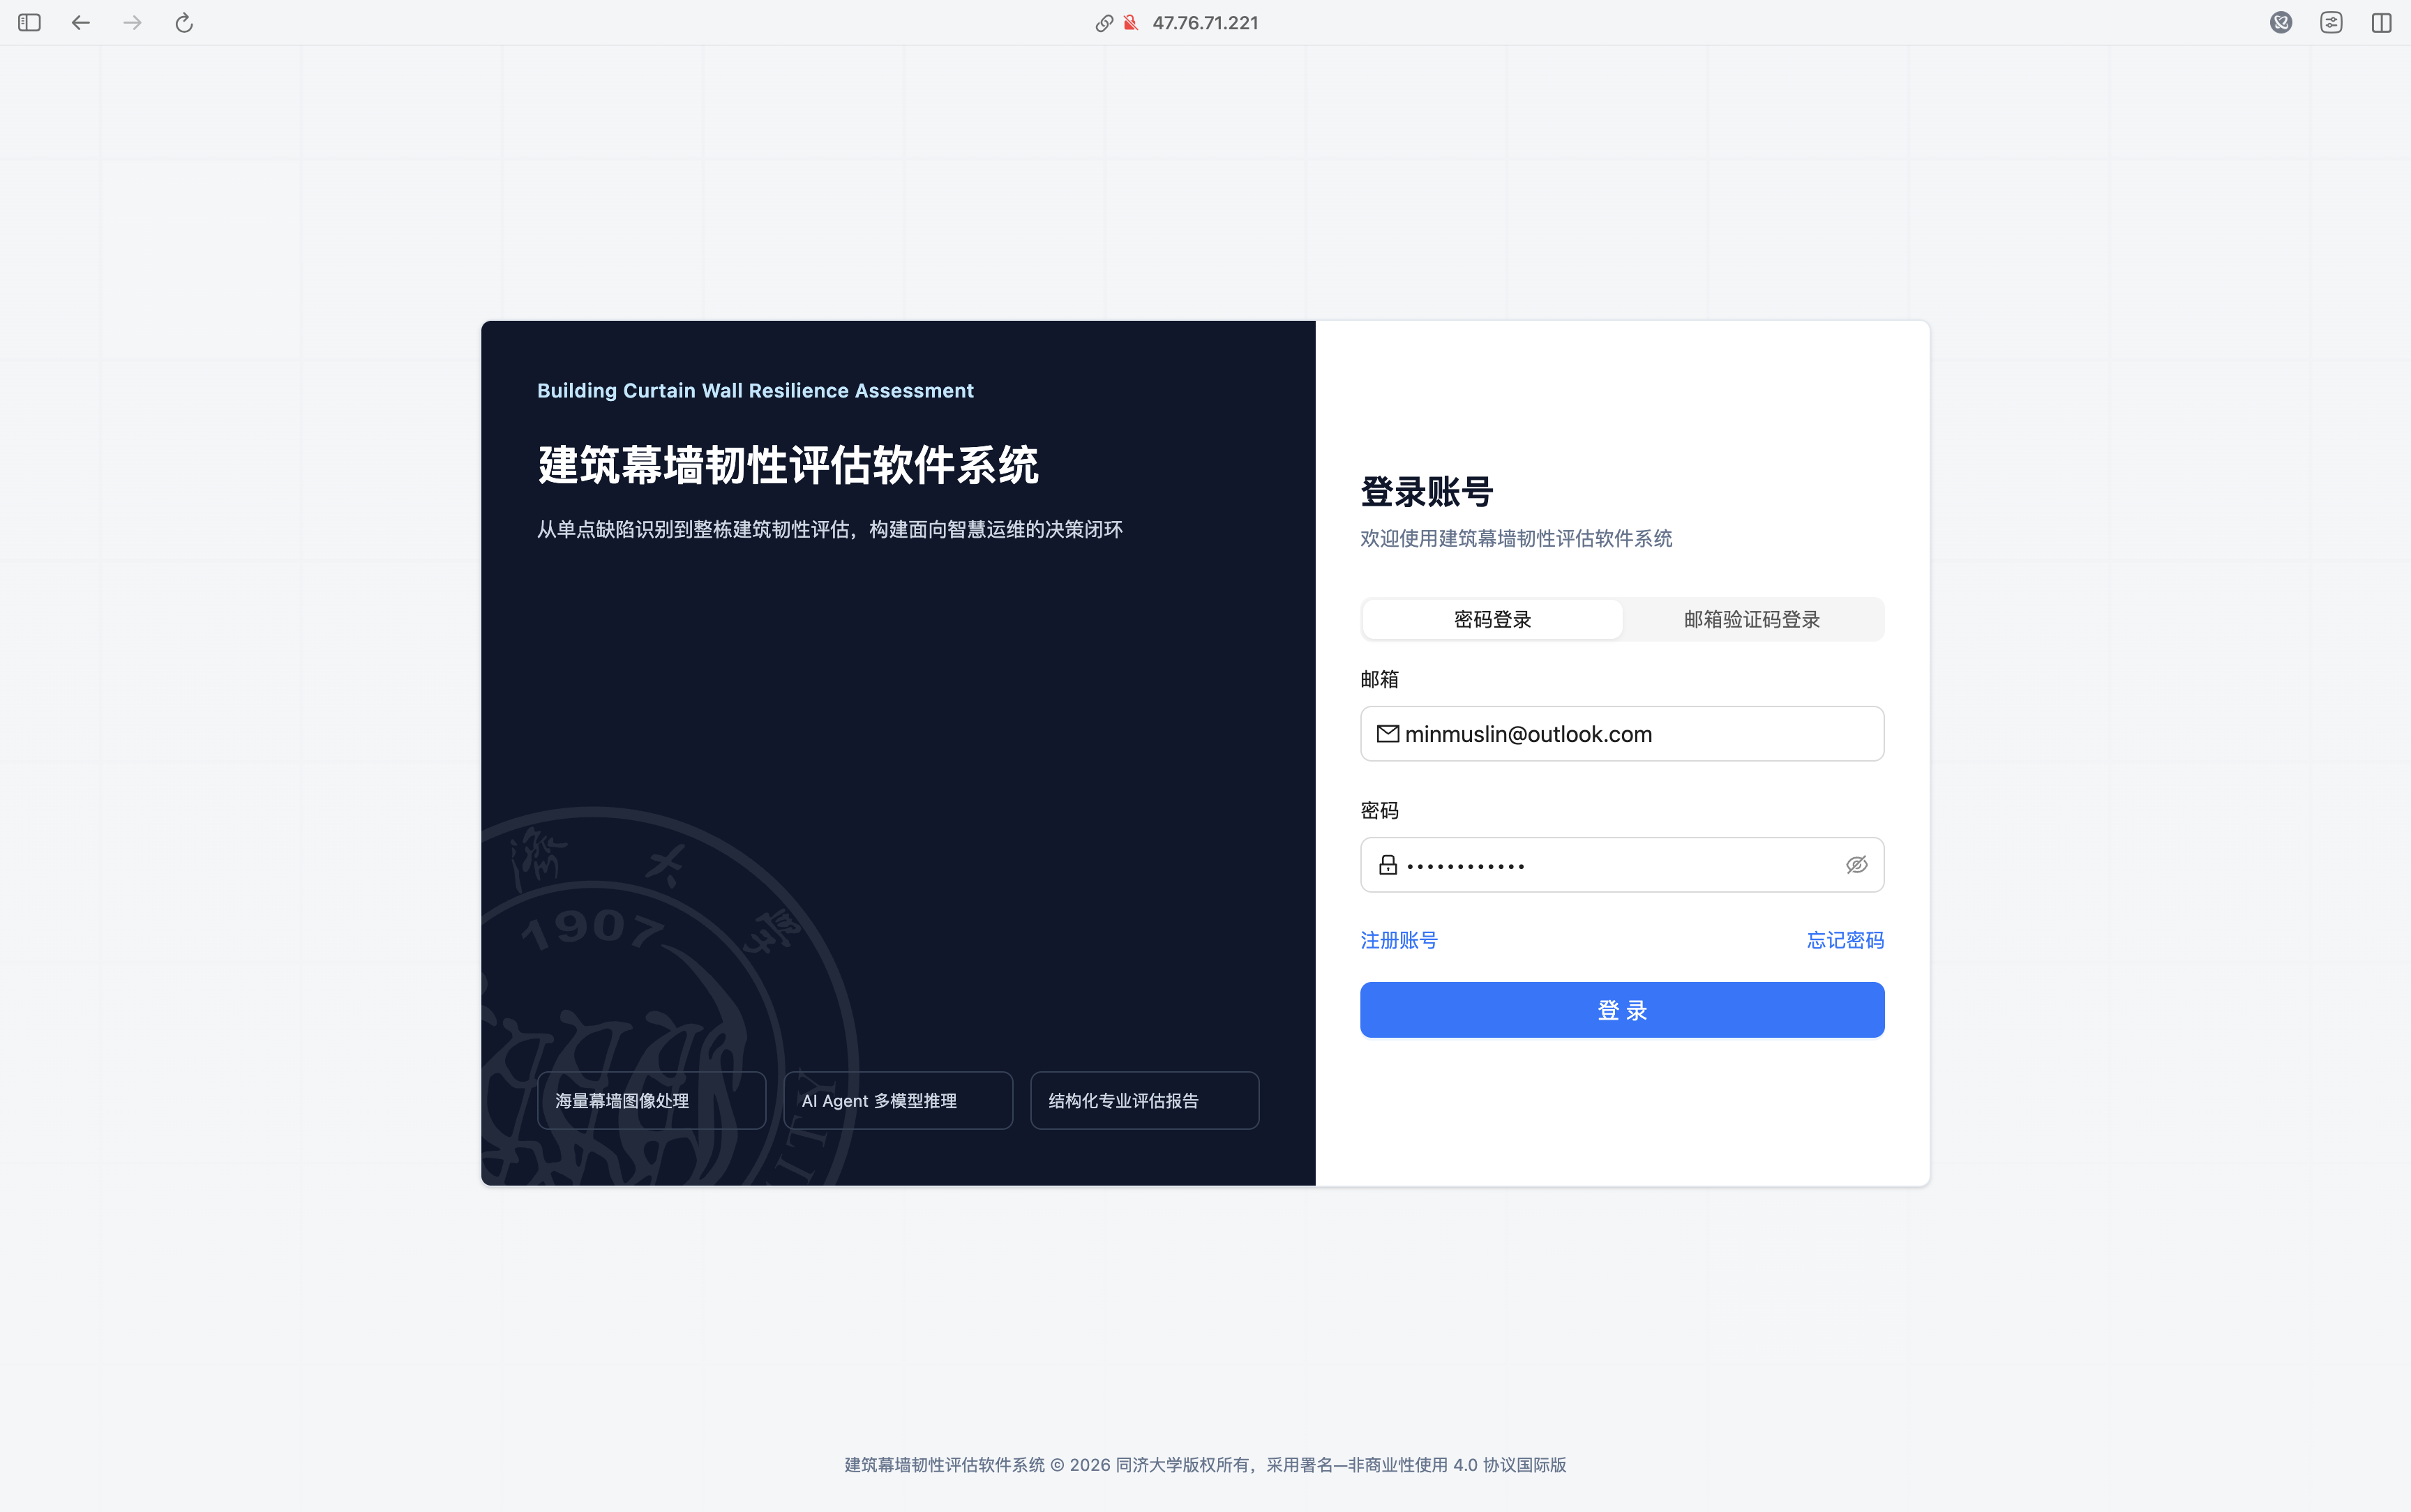
\includegraphics[width=0.95\textwidth]{figures/showcase_01_user_login.png}
  \caption{用户登录界面}
  \label{fig:validation-showcase-user-login}
\end{figure}

\begin{figure}[!htbp]
  \centering
  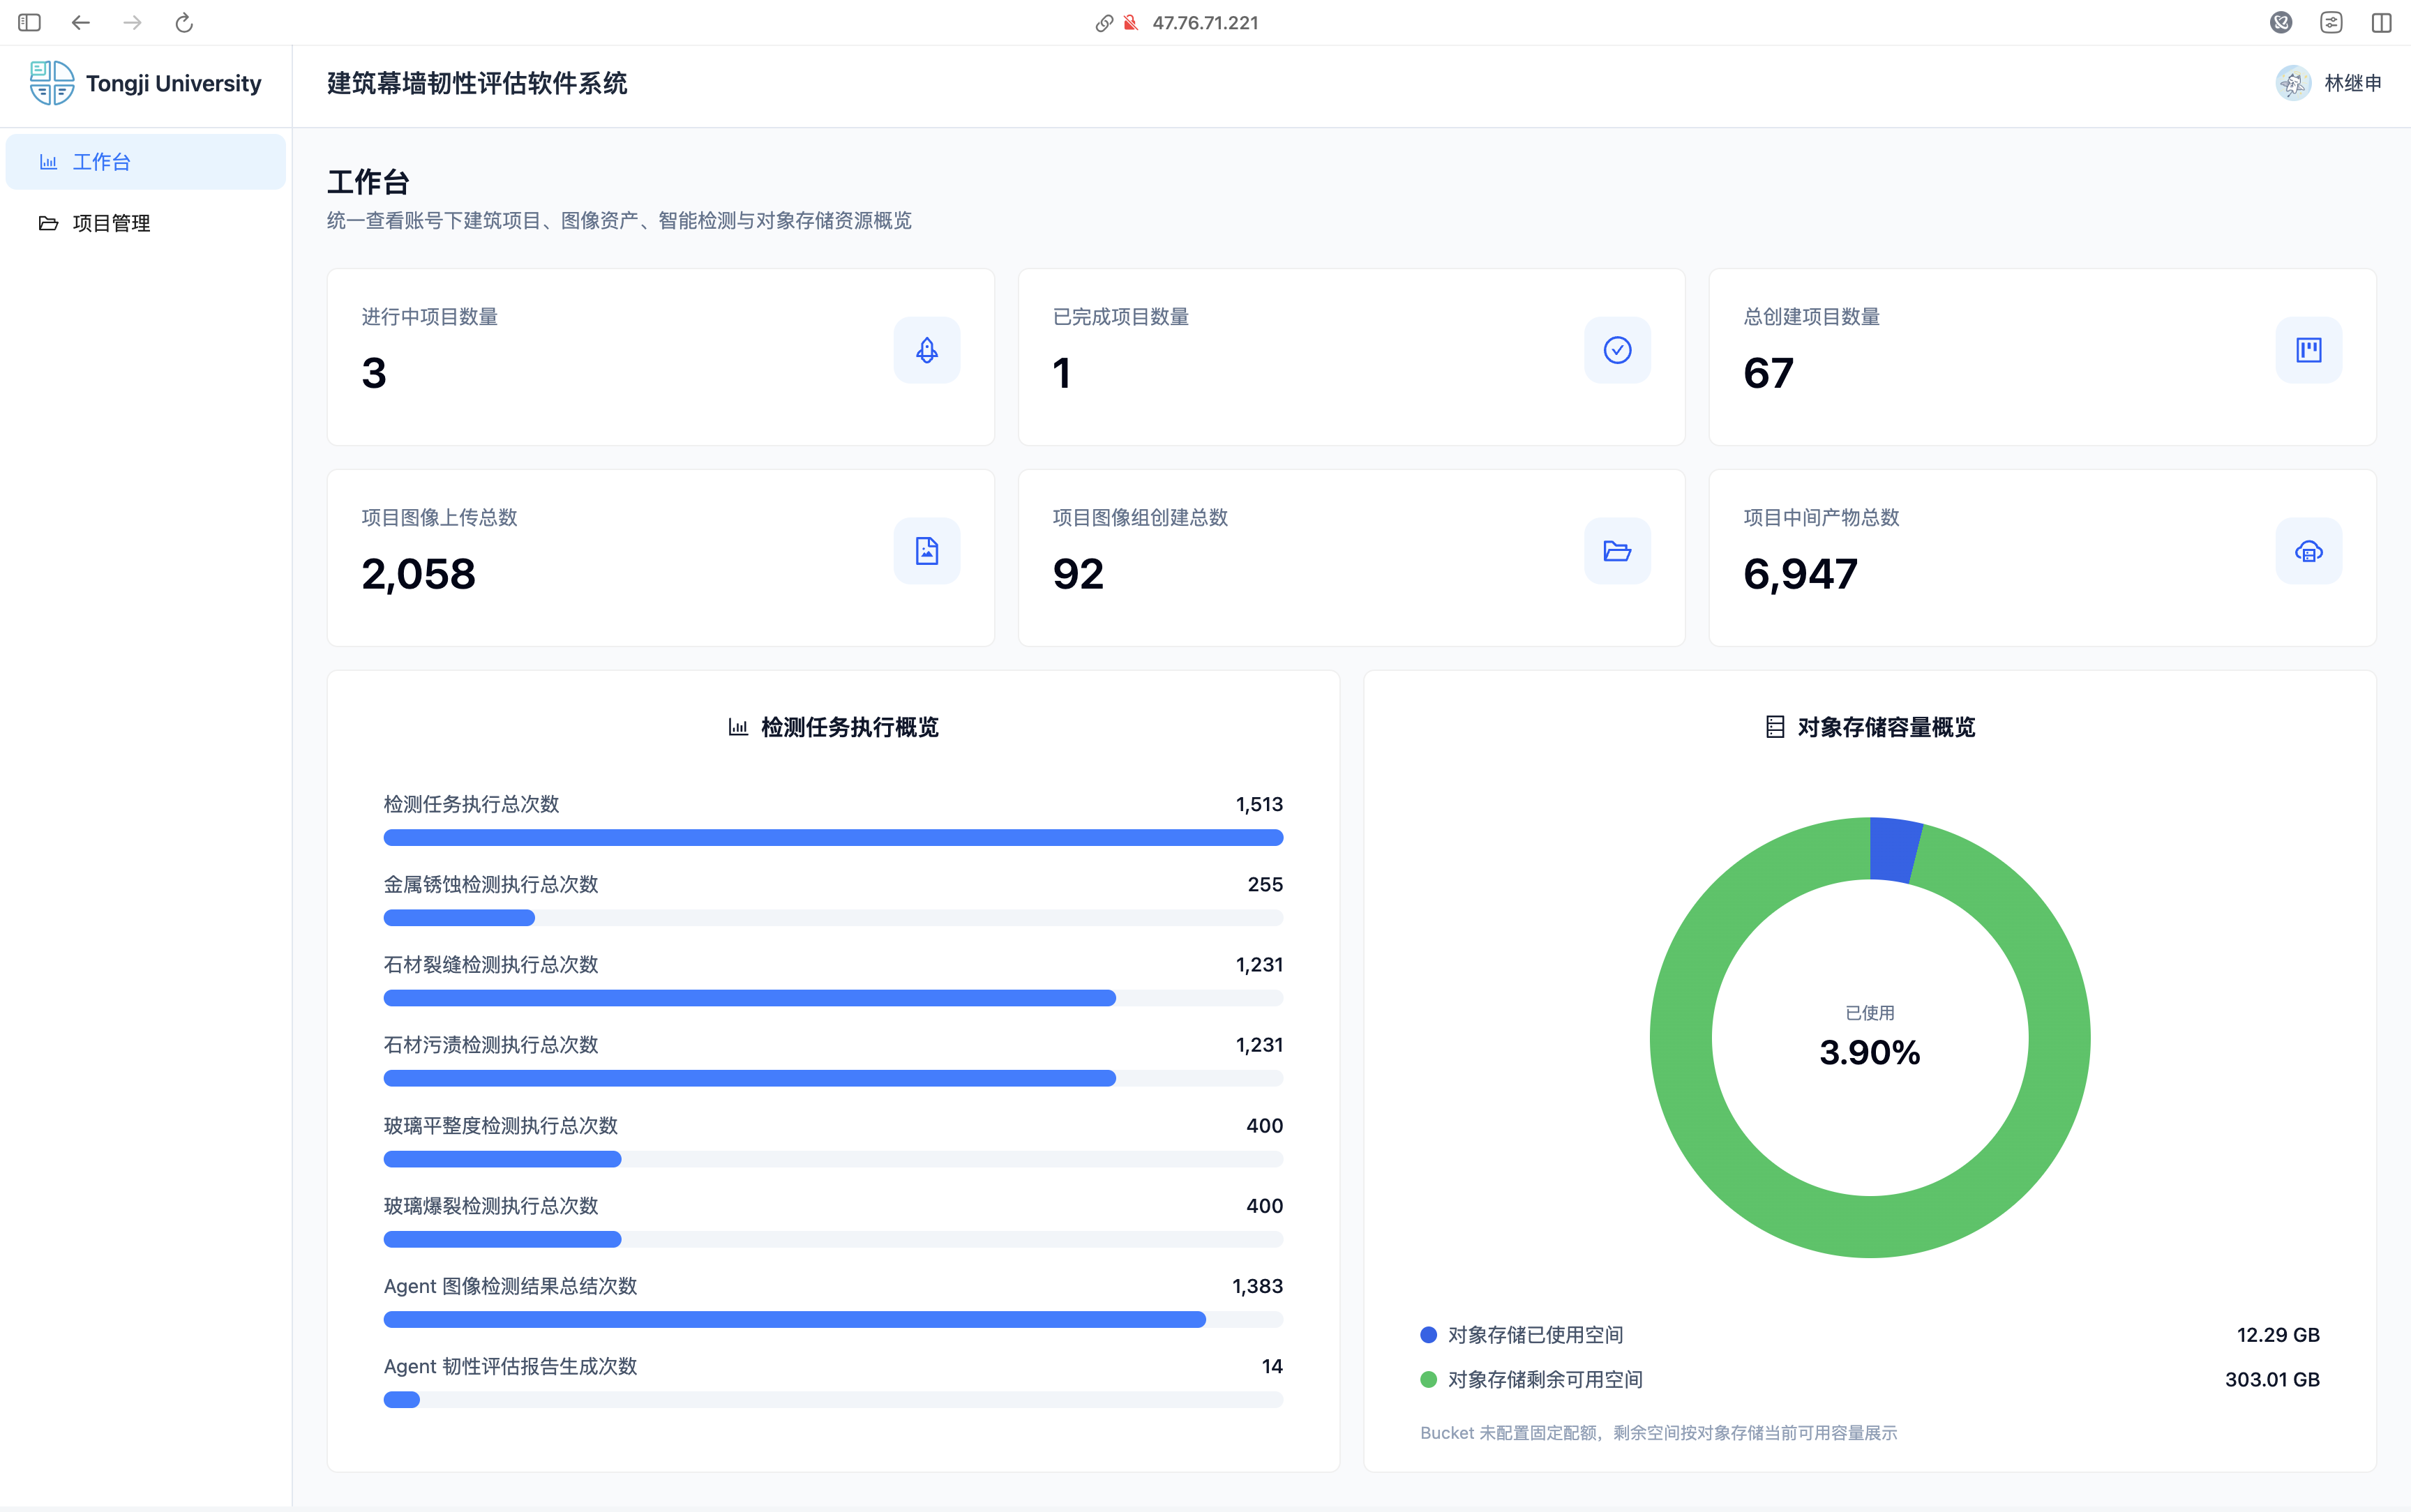
\includegraphics[width=0.95\textwidth]{figures/showcase_02_dashboard.png}
  \caption{工作台数据概览界面}
  \label{fig:validation-showcase-dashboard}
\end{figure}

\begin{figure}[!htbp]
  \centering
  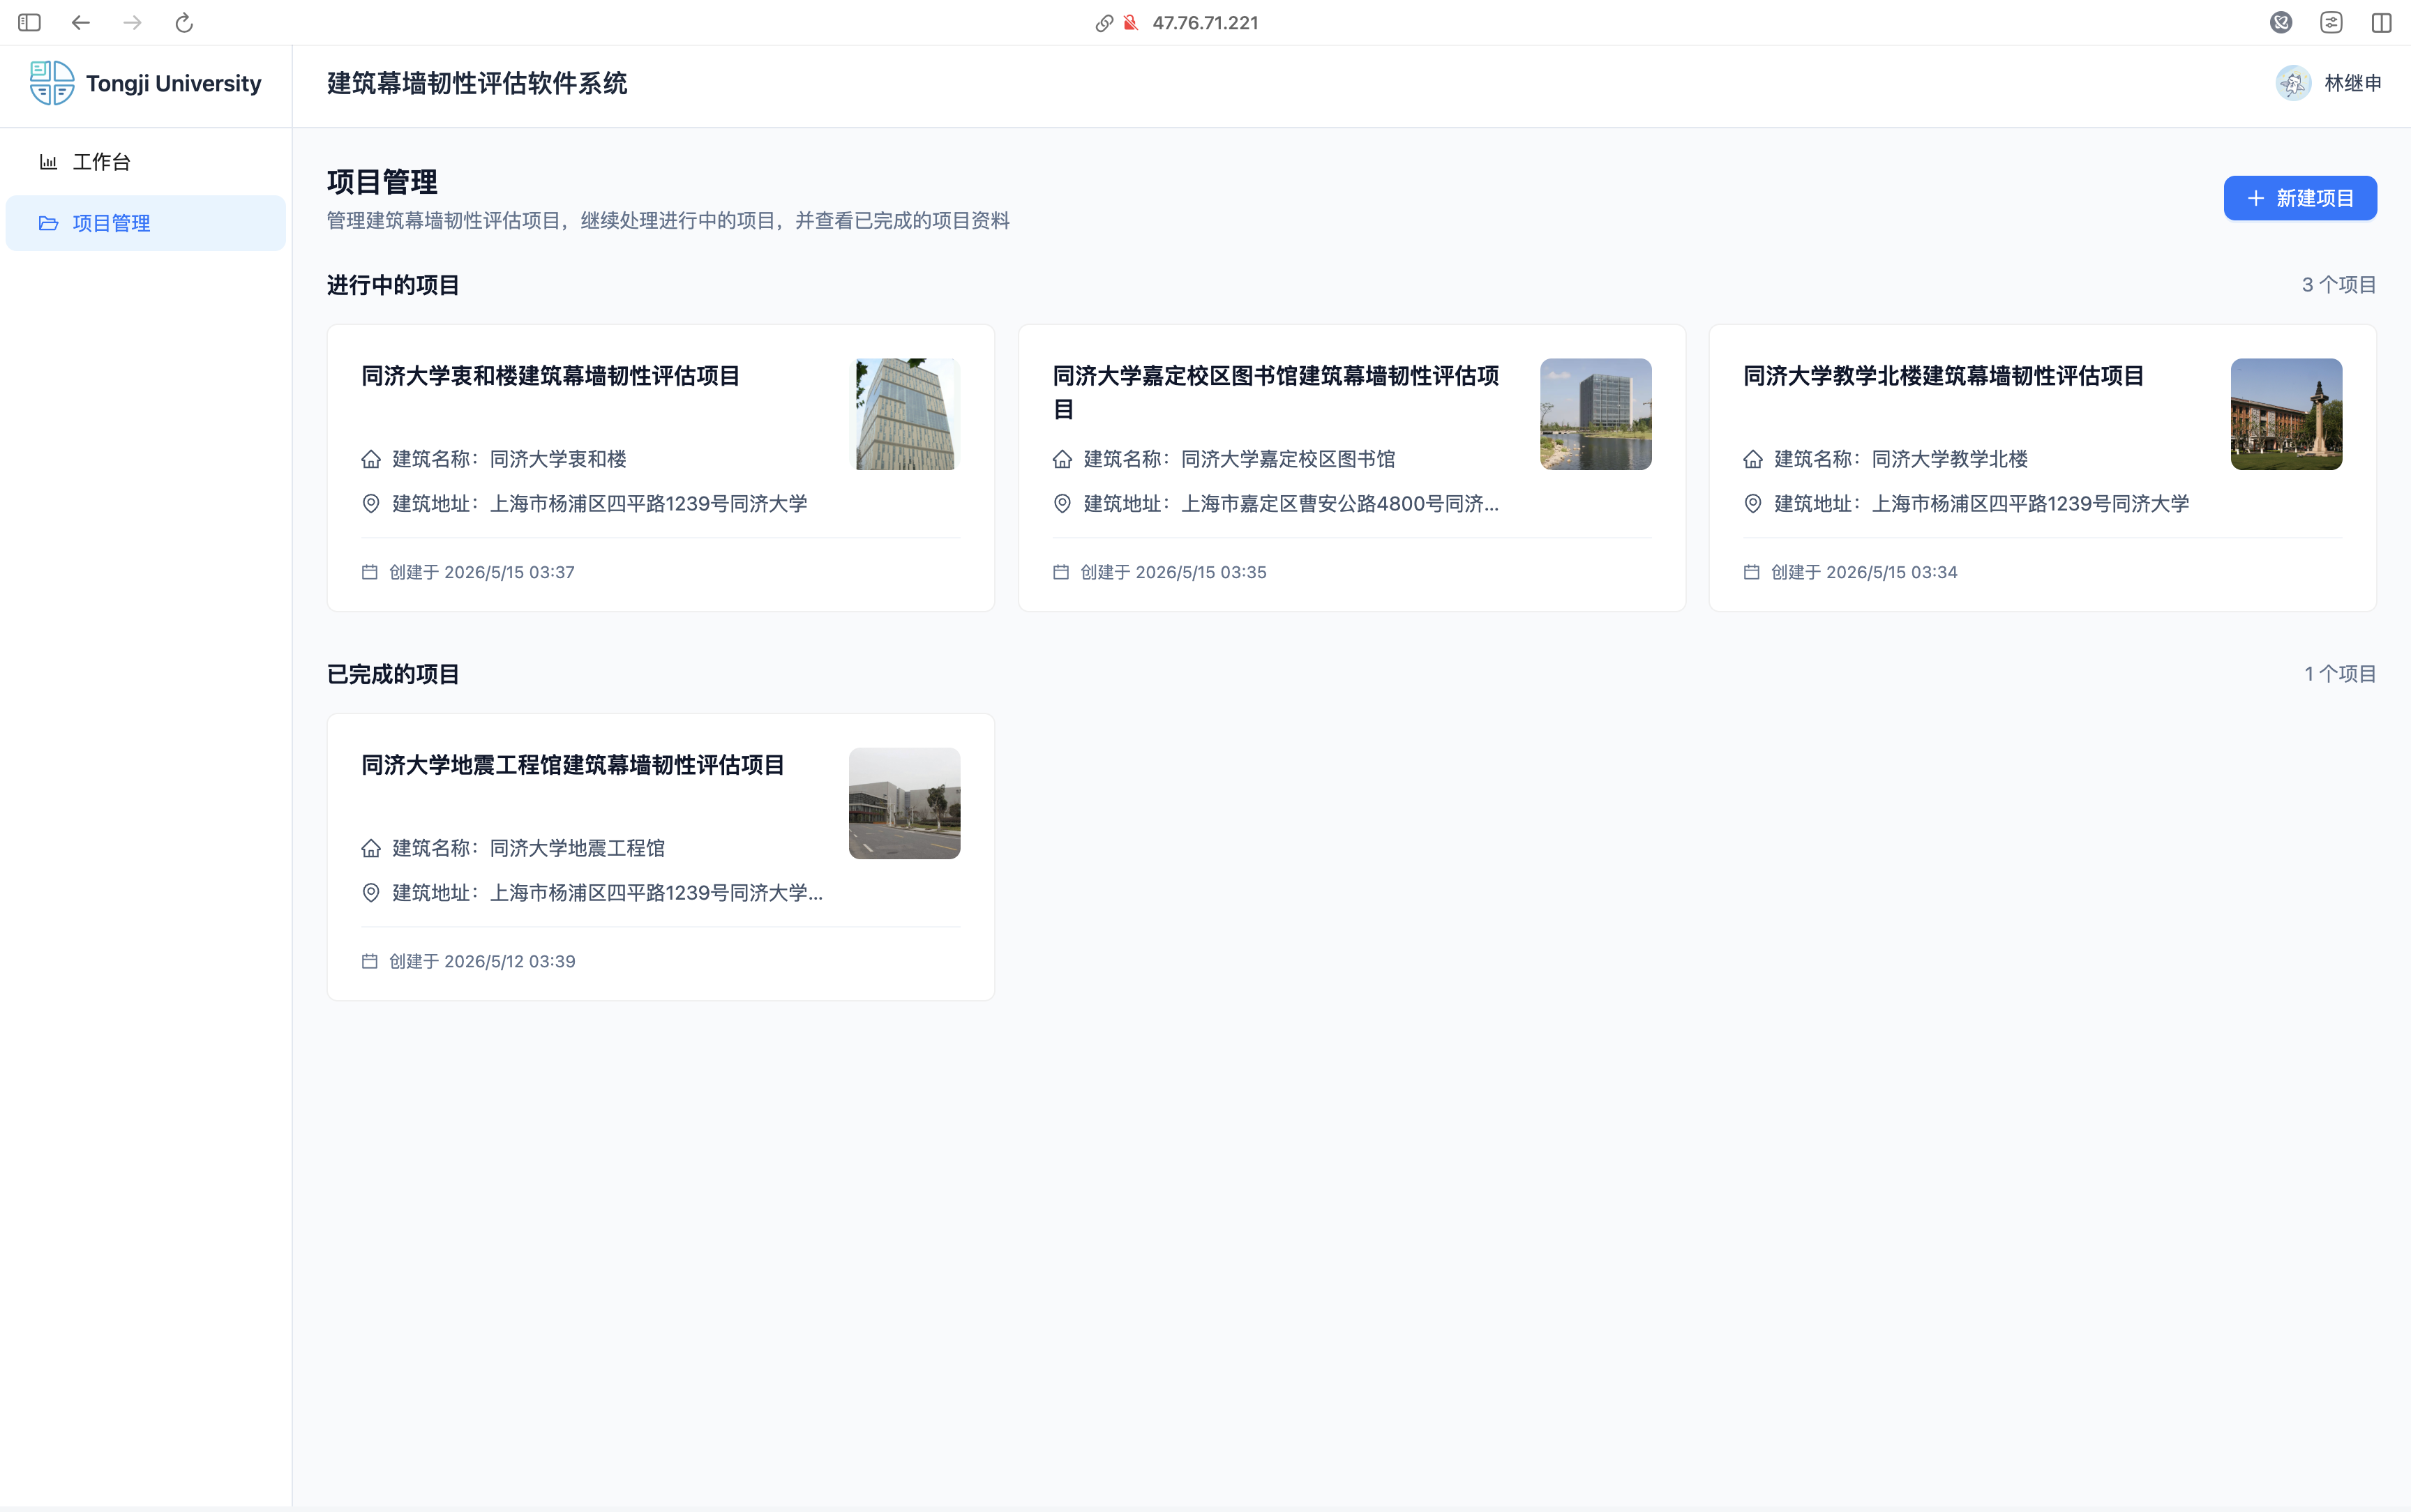
\includegraphics[width=0.95\textwidth]{figures/showcase_03_project_management.png}
  \caption{项目管理界面}
  \label{fig:validation-showcase-project-management}
\end{figure}

\begin{figure}[!htbp]
  \centering
  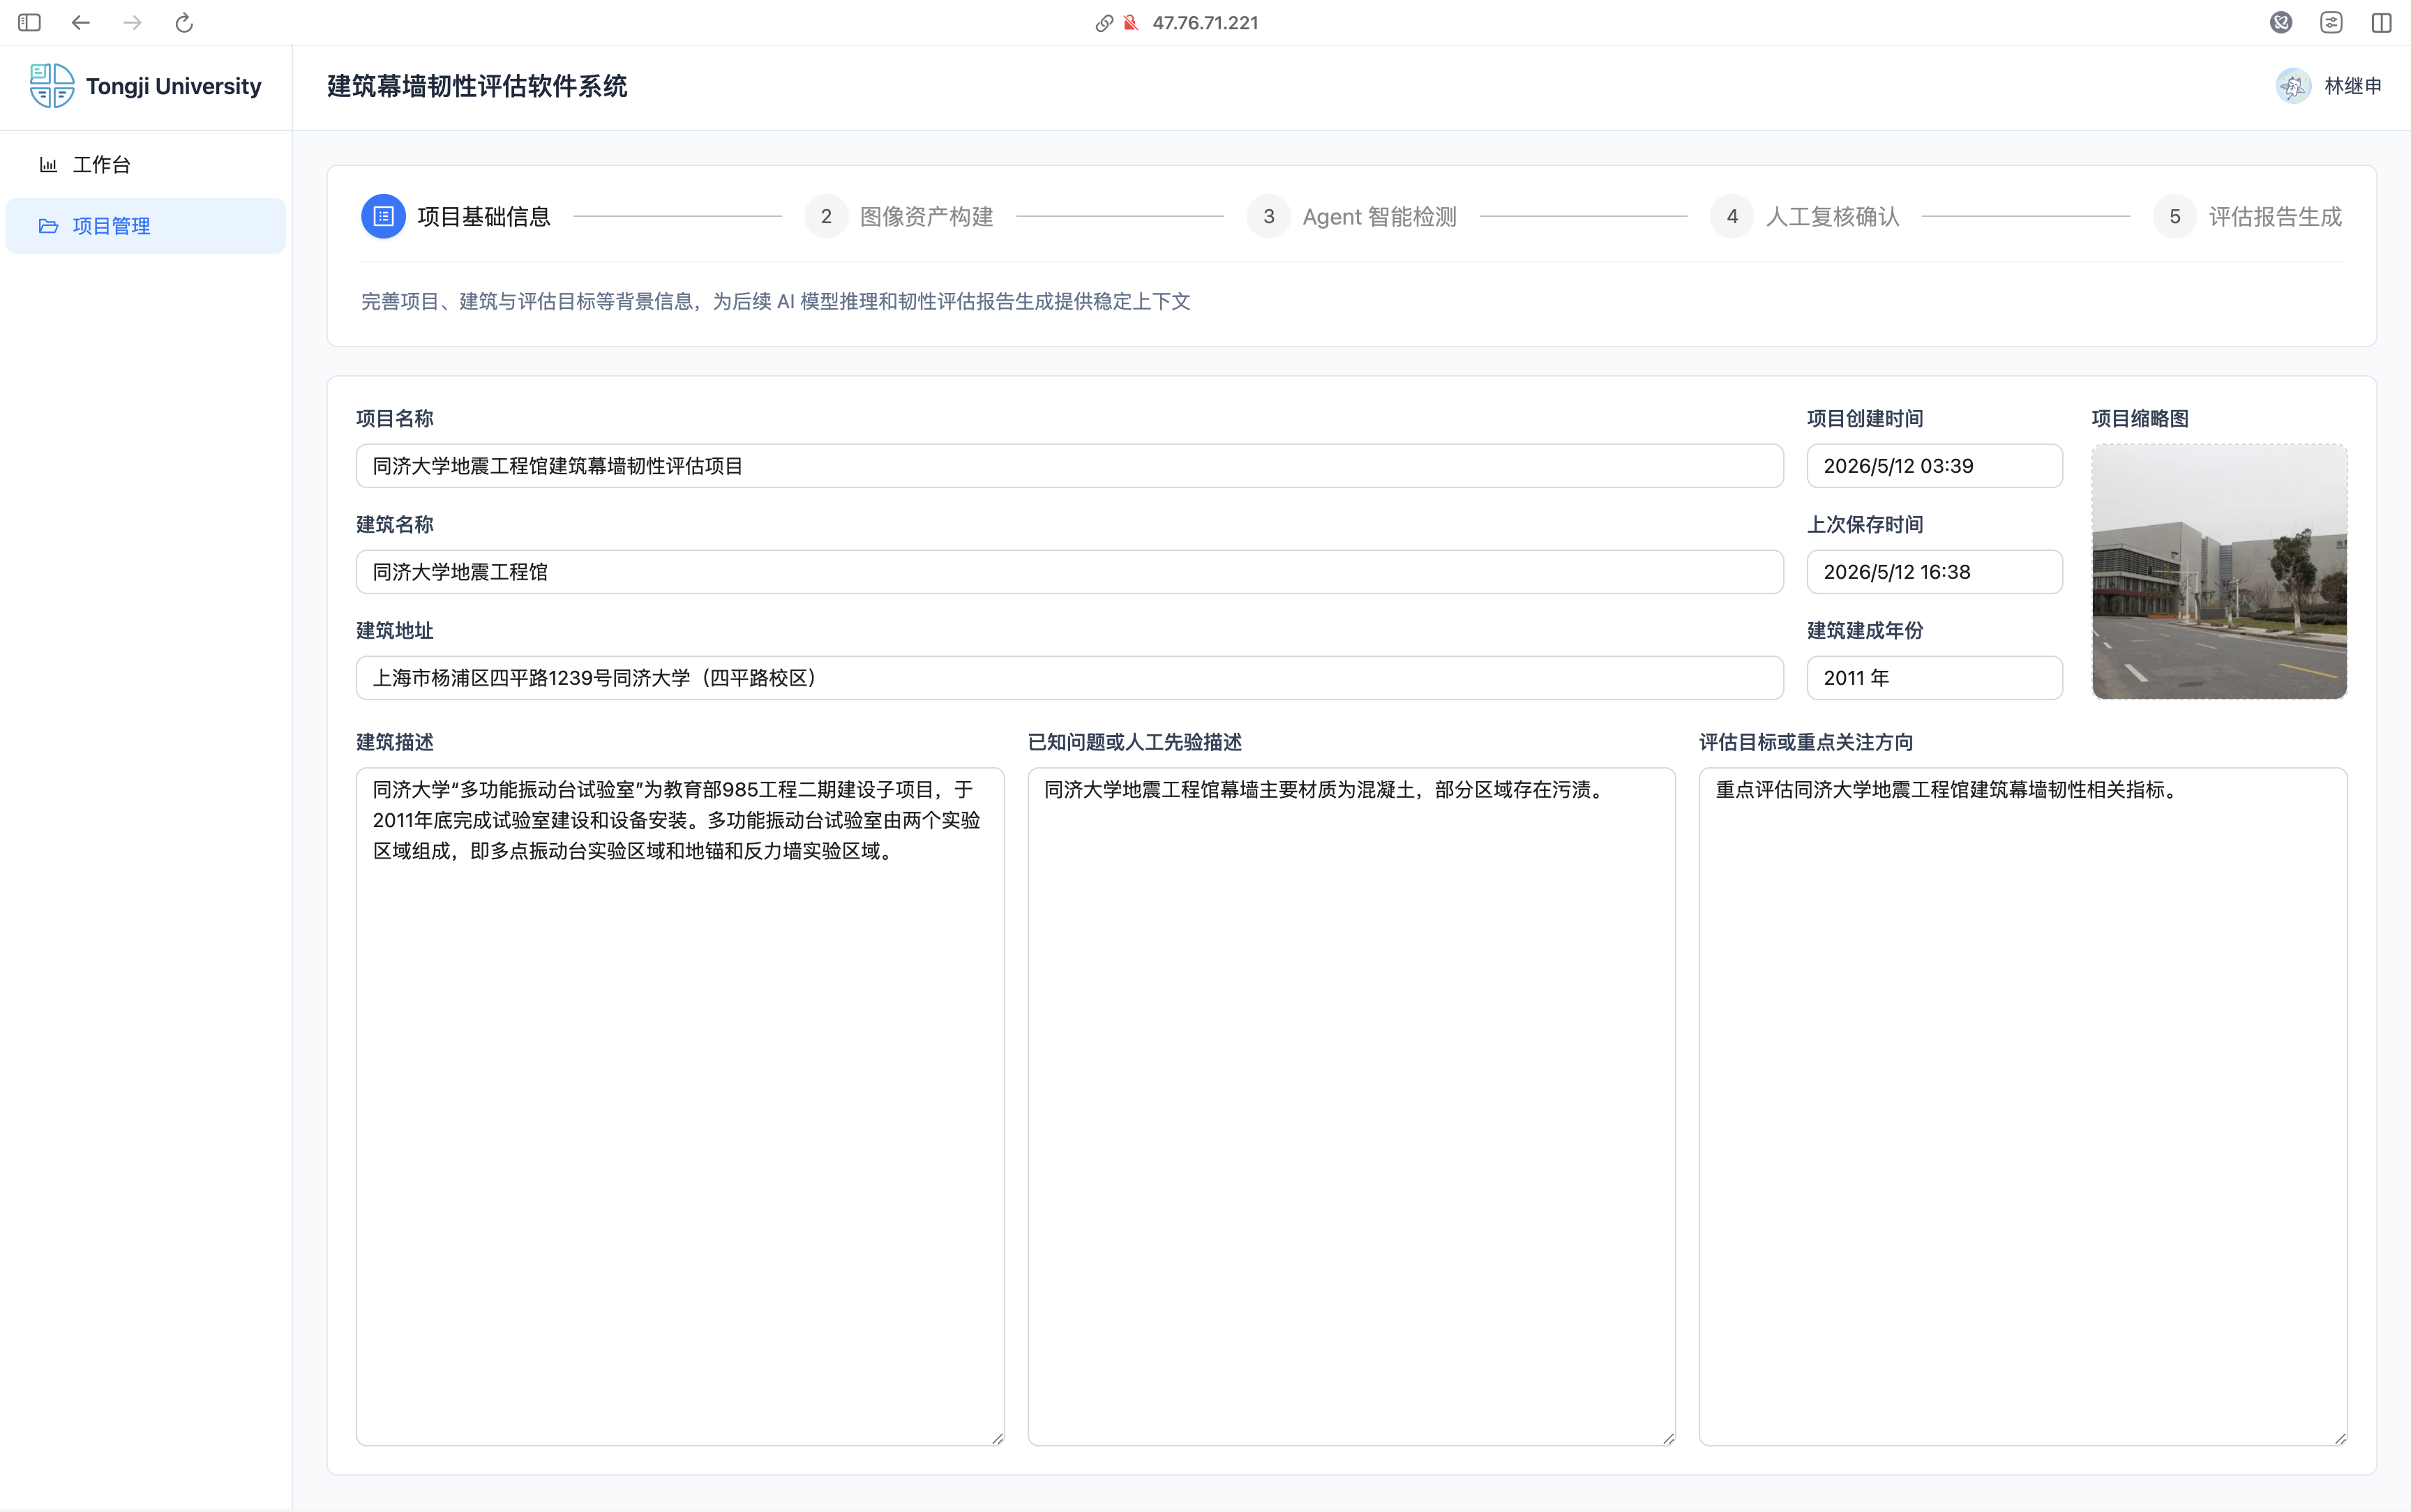
\includegraphics[width=0.95\textwidth]{figures/showcase_04_project_profile.png}
  \caption{项目基础信息界面}
  \label{fig:validation-showcase-project-profile}
\end{figure}

\begin{figure}[!htbp]
  \centering
  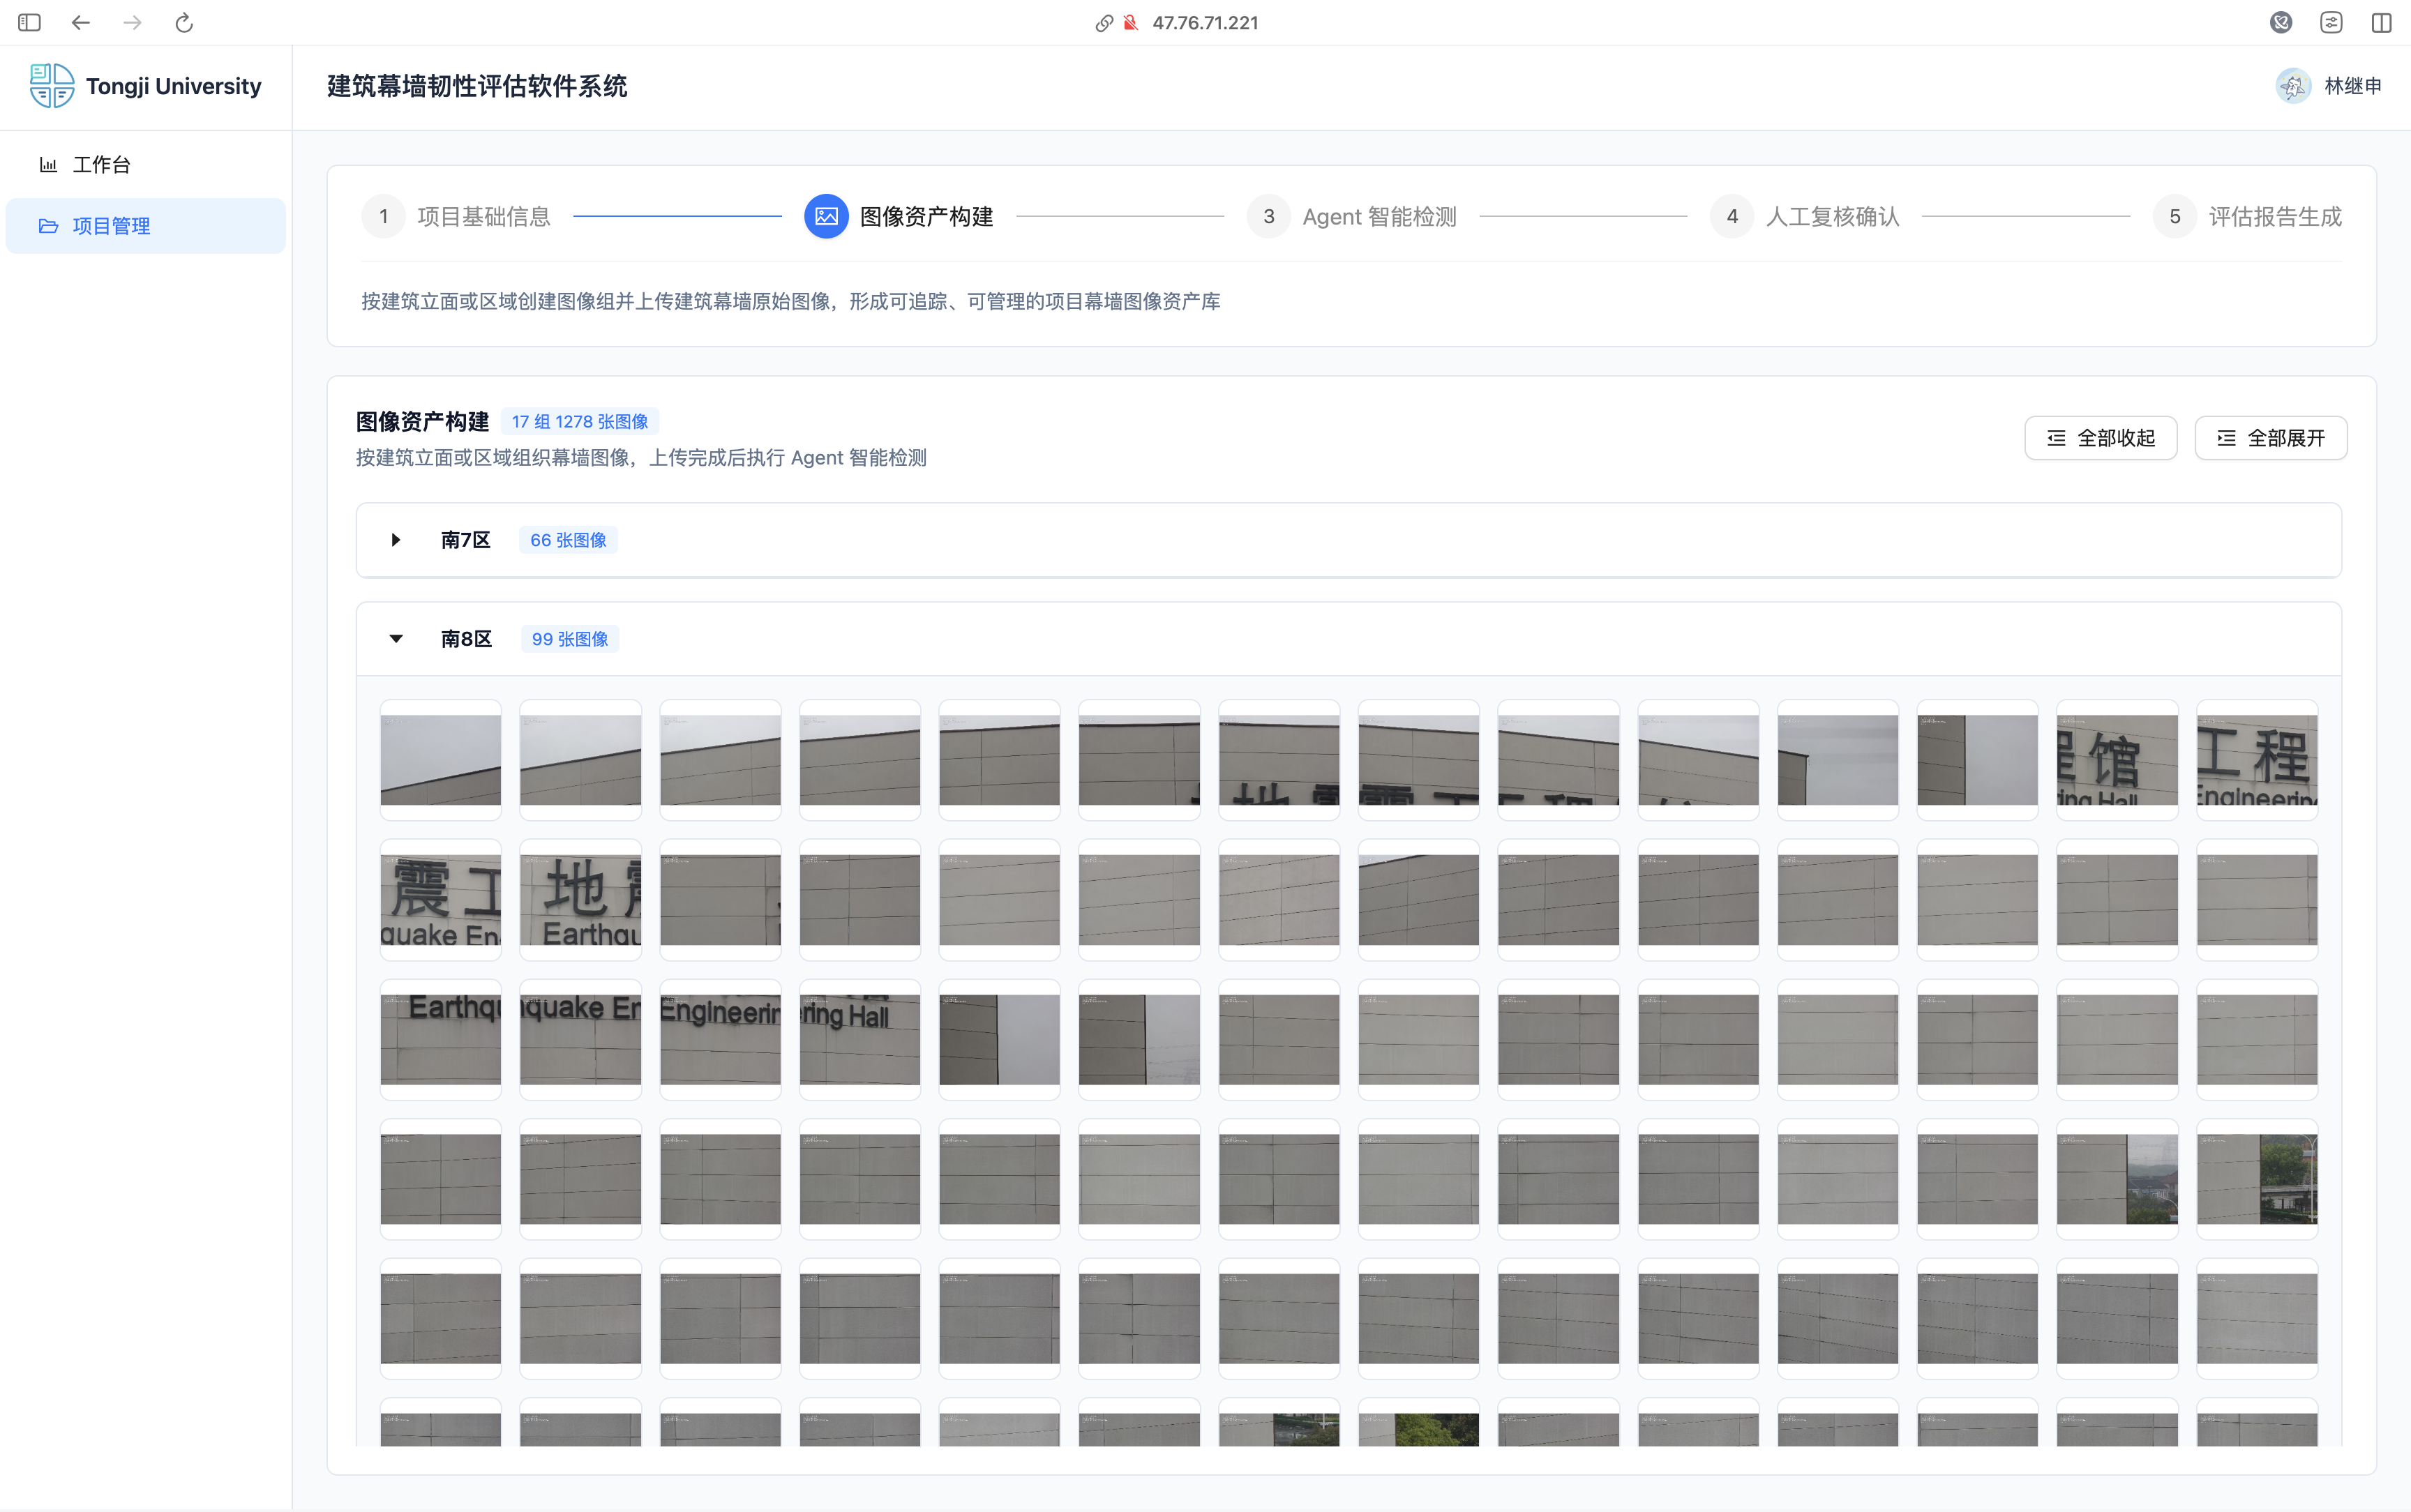
\includegraphics[width=0.95\textwidth]{figures/showcase_05_project_assets.png}
  \caption{图像资产构建界面}
  \label{fig:validation-showcase-project-assets}
\end{figure}

\subsection{Agent 自主任务调度方法验证结果}
\label{subsec:validation-agent-scheduling-result-display}

\begin{figure}[!htbp]
  \centering
  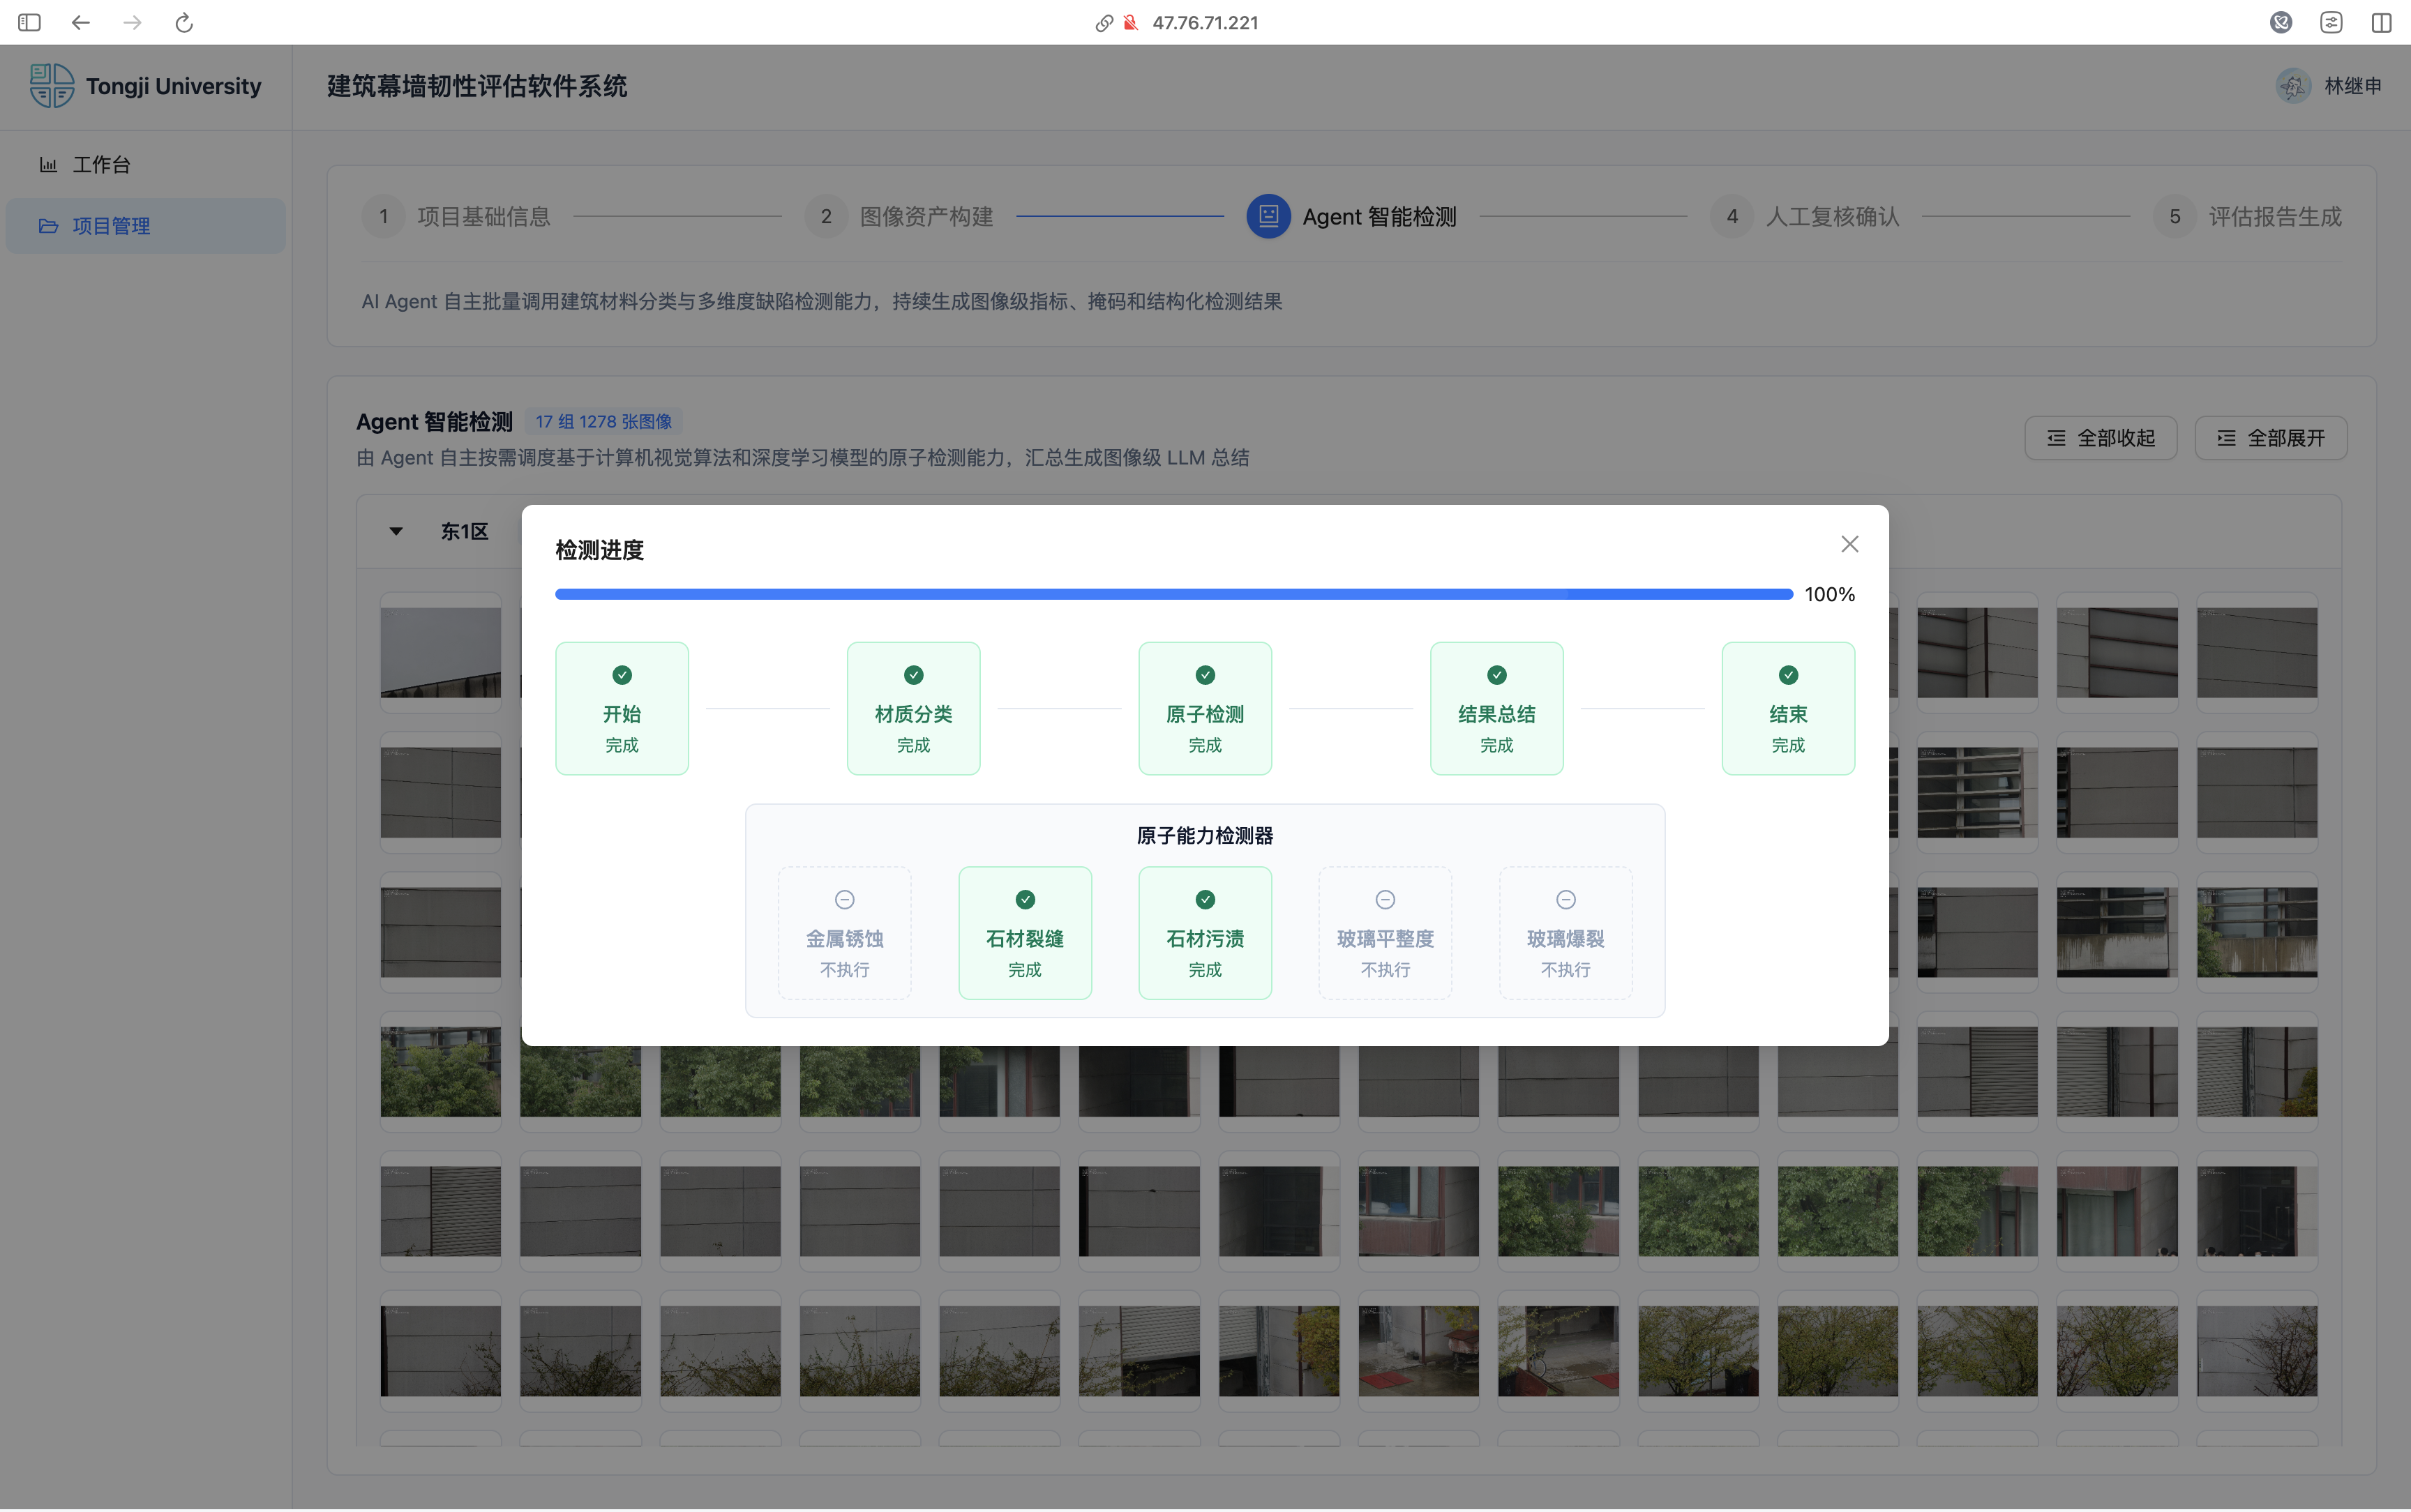
\includegraphics[width=0.95\textwidth]{figures/showcase_06_project_detection.png}
  \caption{Agent 智能检测界面}
  \label{fig:validation-showcase-project-detection}
\end{figure}

\begin{figure}[!htbp]
  \centering
  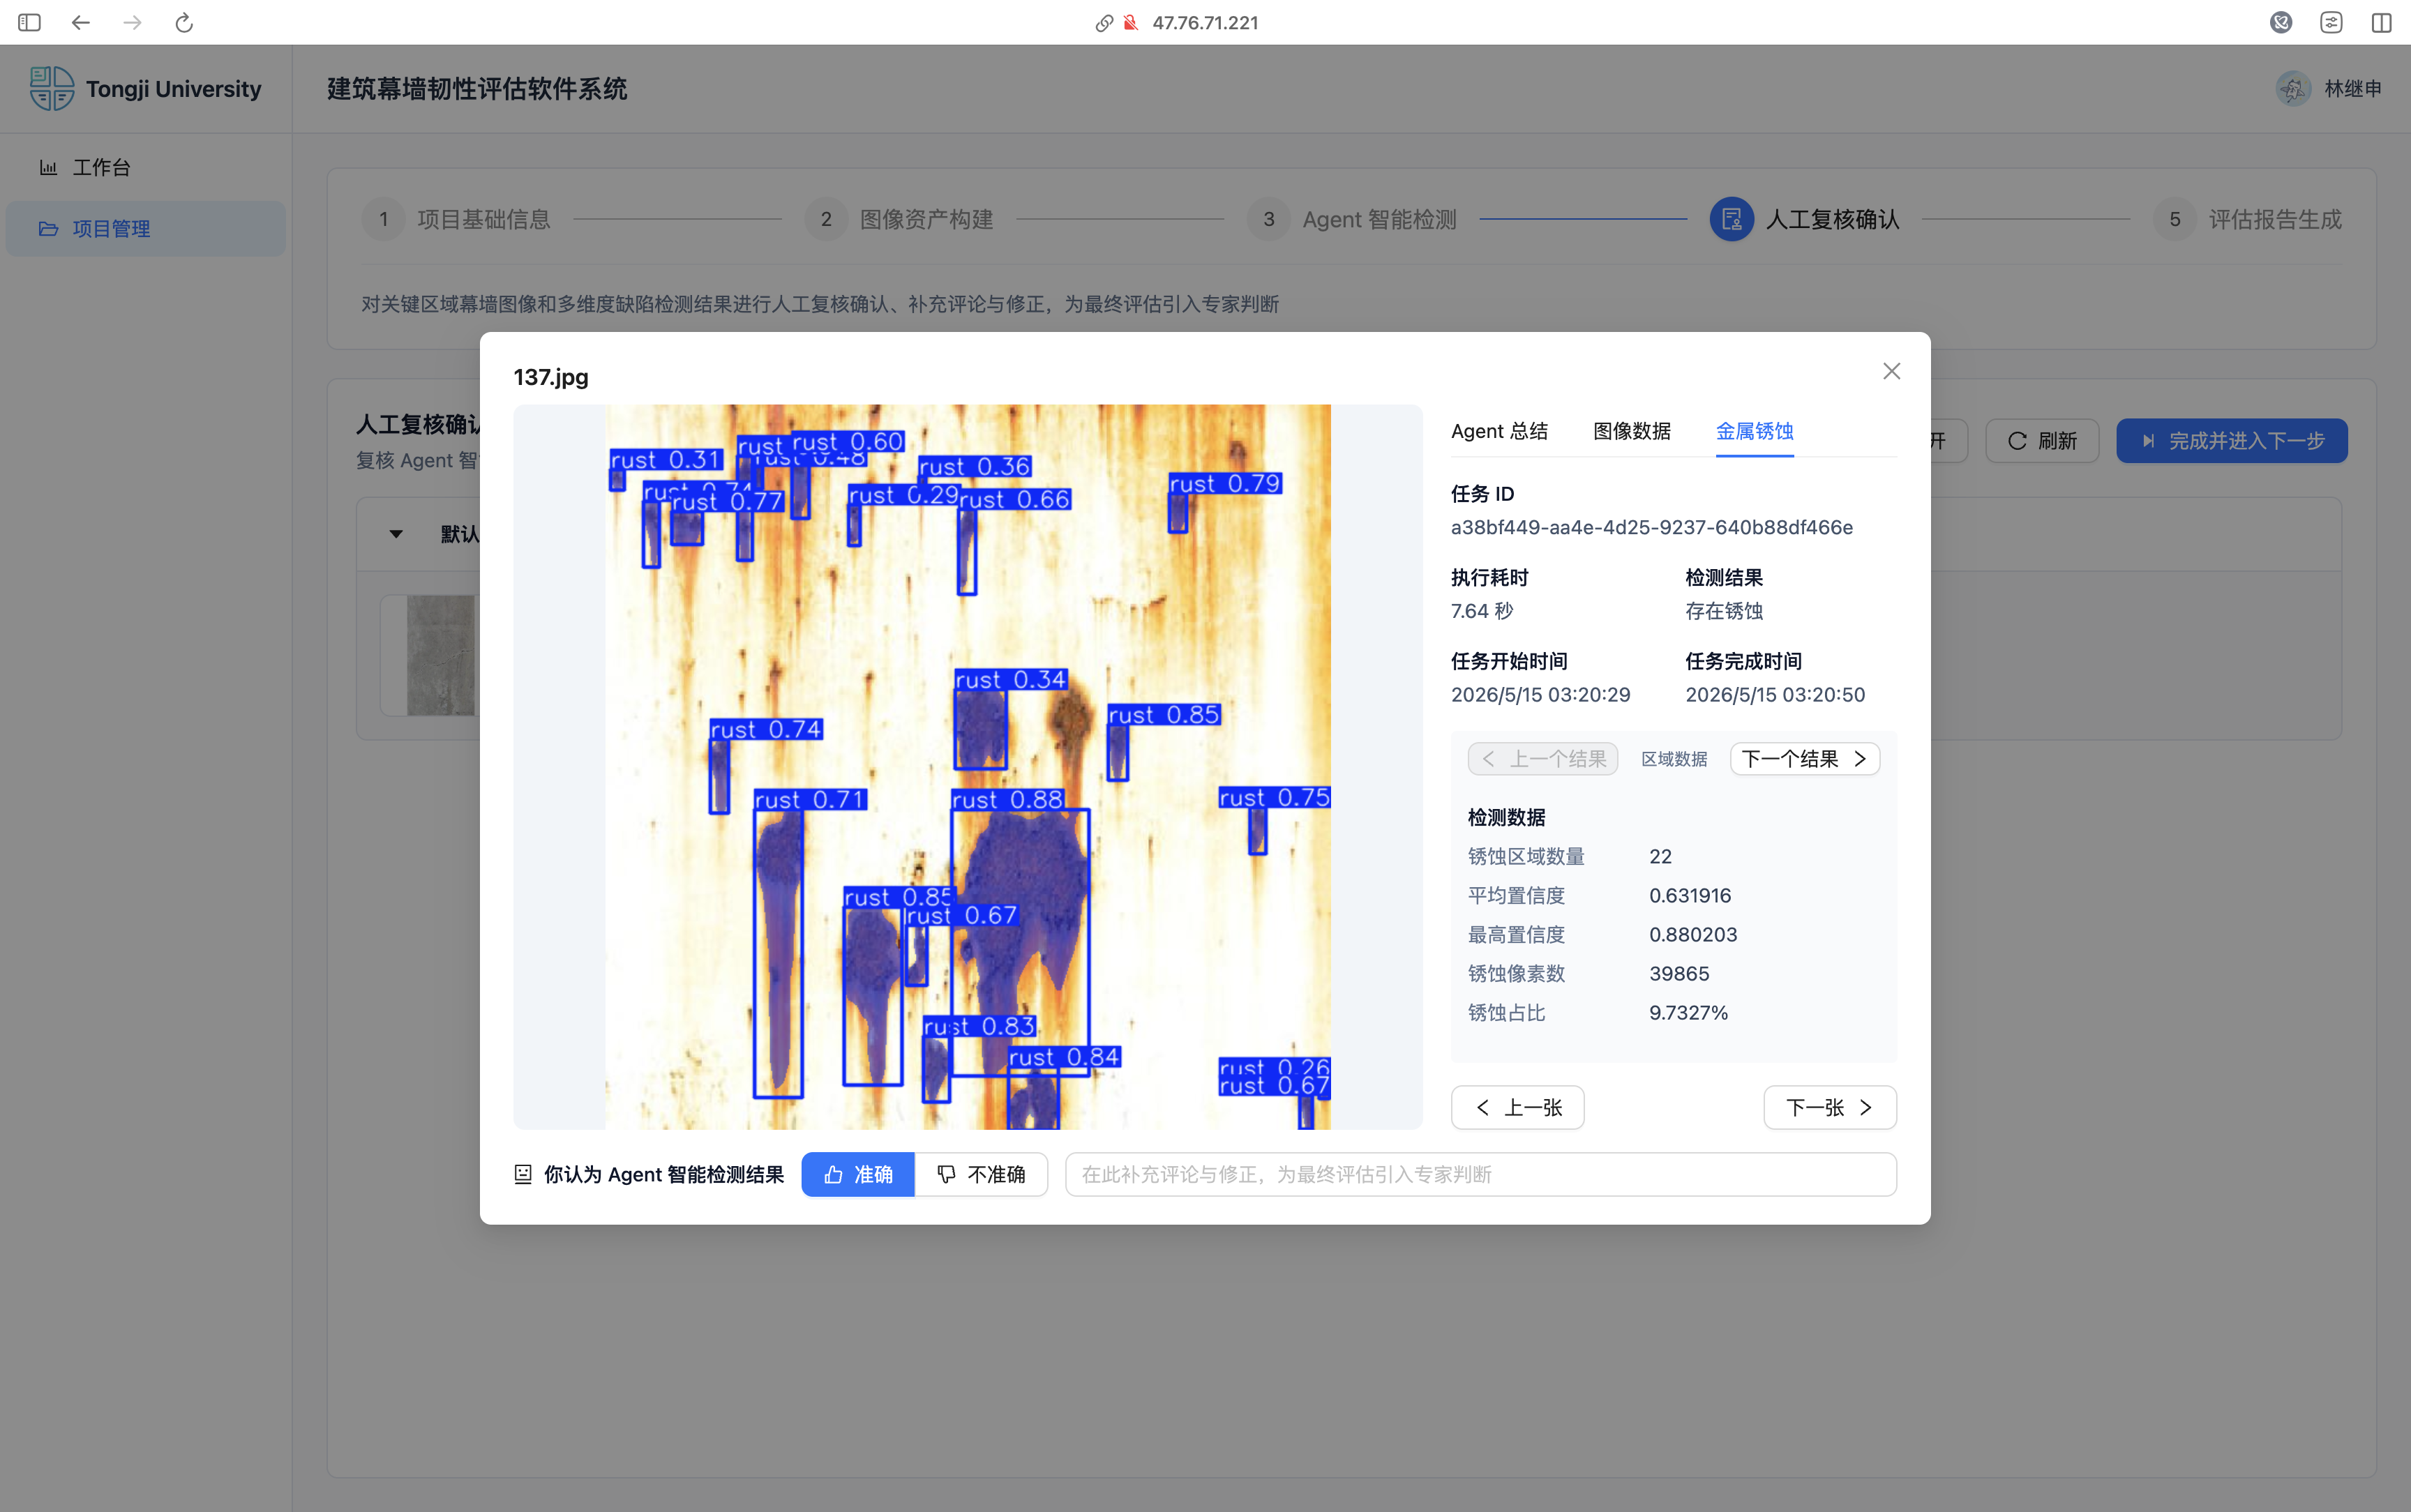
\includegraphics[width=0.95\textwidth]{figures/showcase_07_corrosion_detection.png}
  \caption{金属锈蚀检测结果界面}
  \label{fig:validation-showcase-corrosion-detection}
\end{figure}

\begin{figure}[!htbp]
  \centering
  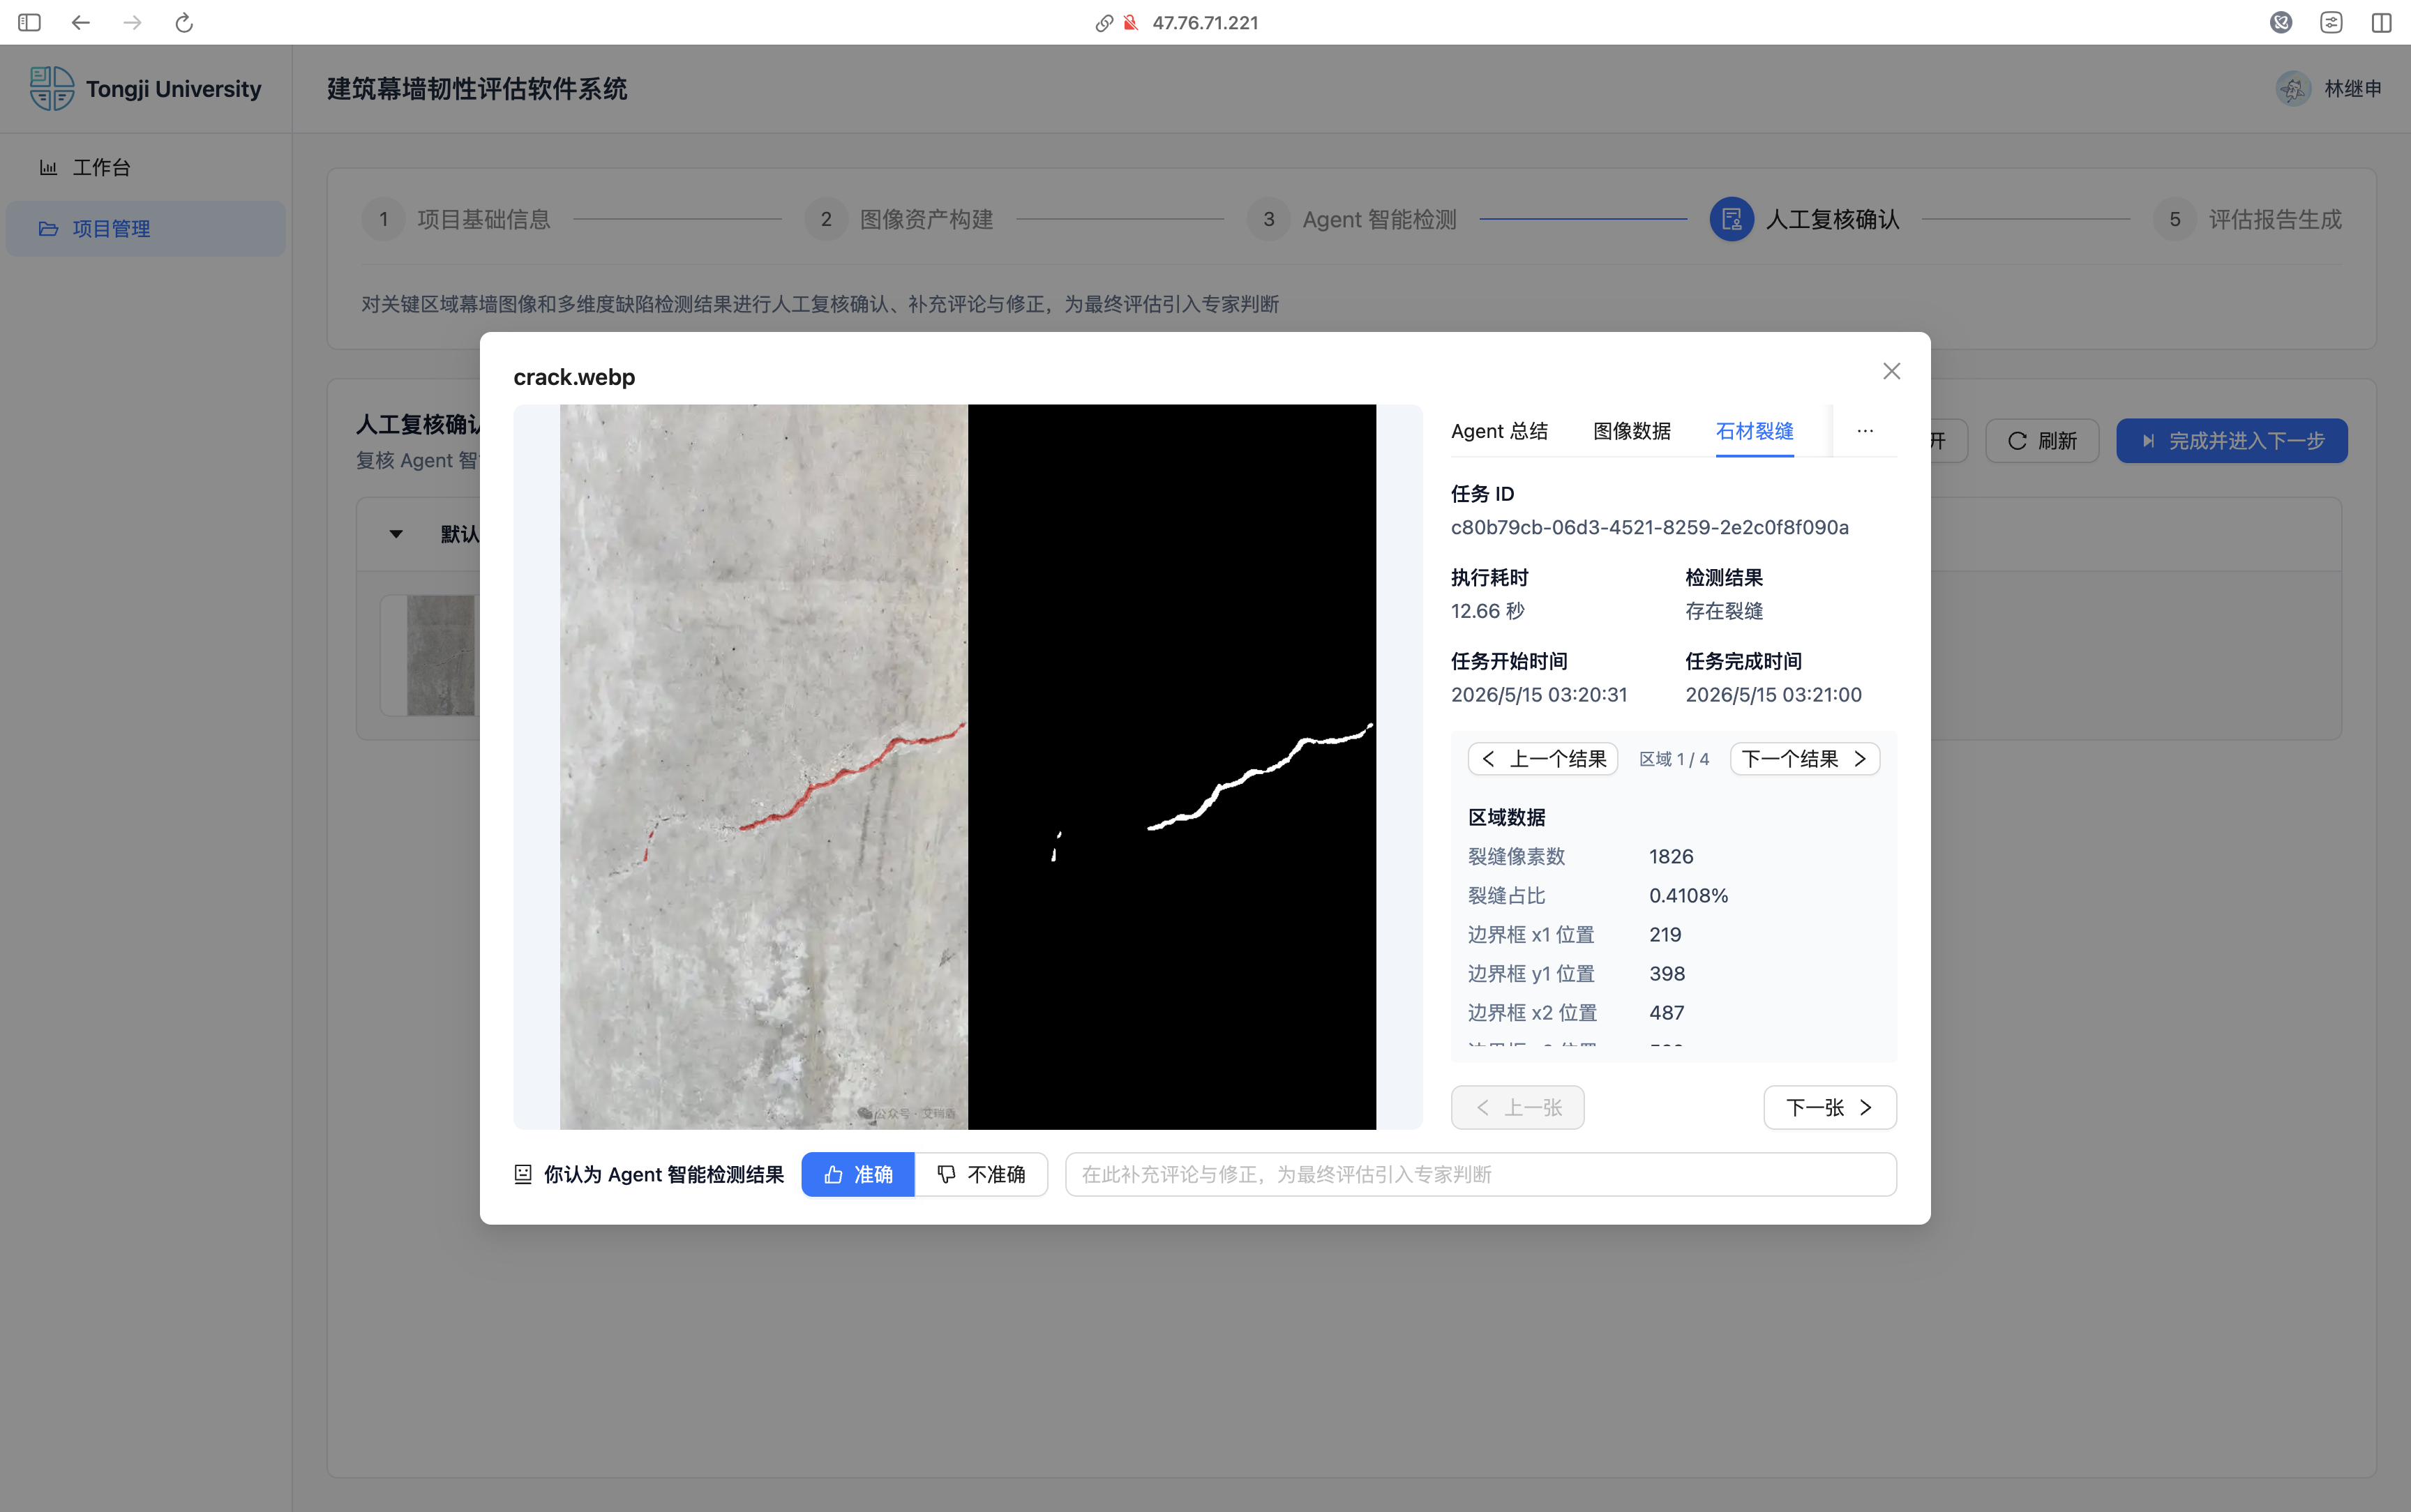
\includegraphics[width=0.95\textwidth]{figures/showcase_08_crack_detection.png}
  \caption{石材裂缝检测结果界面}
  \label{fig:validation-showcase-crack-detection}
\end{figure}

\begin{figure}[!htbp]
  \centering
  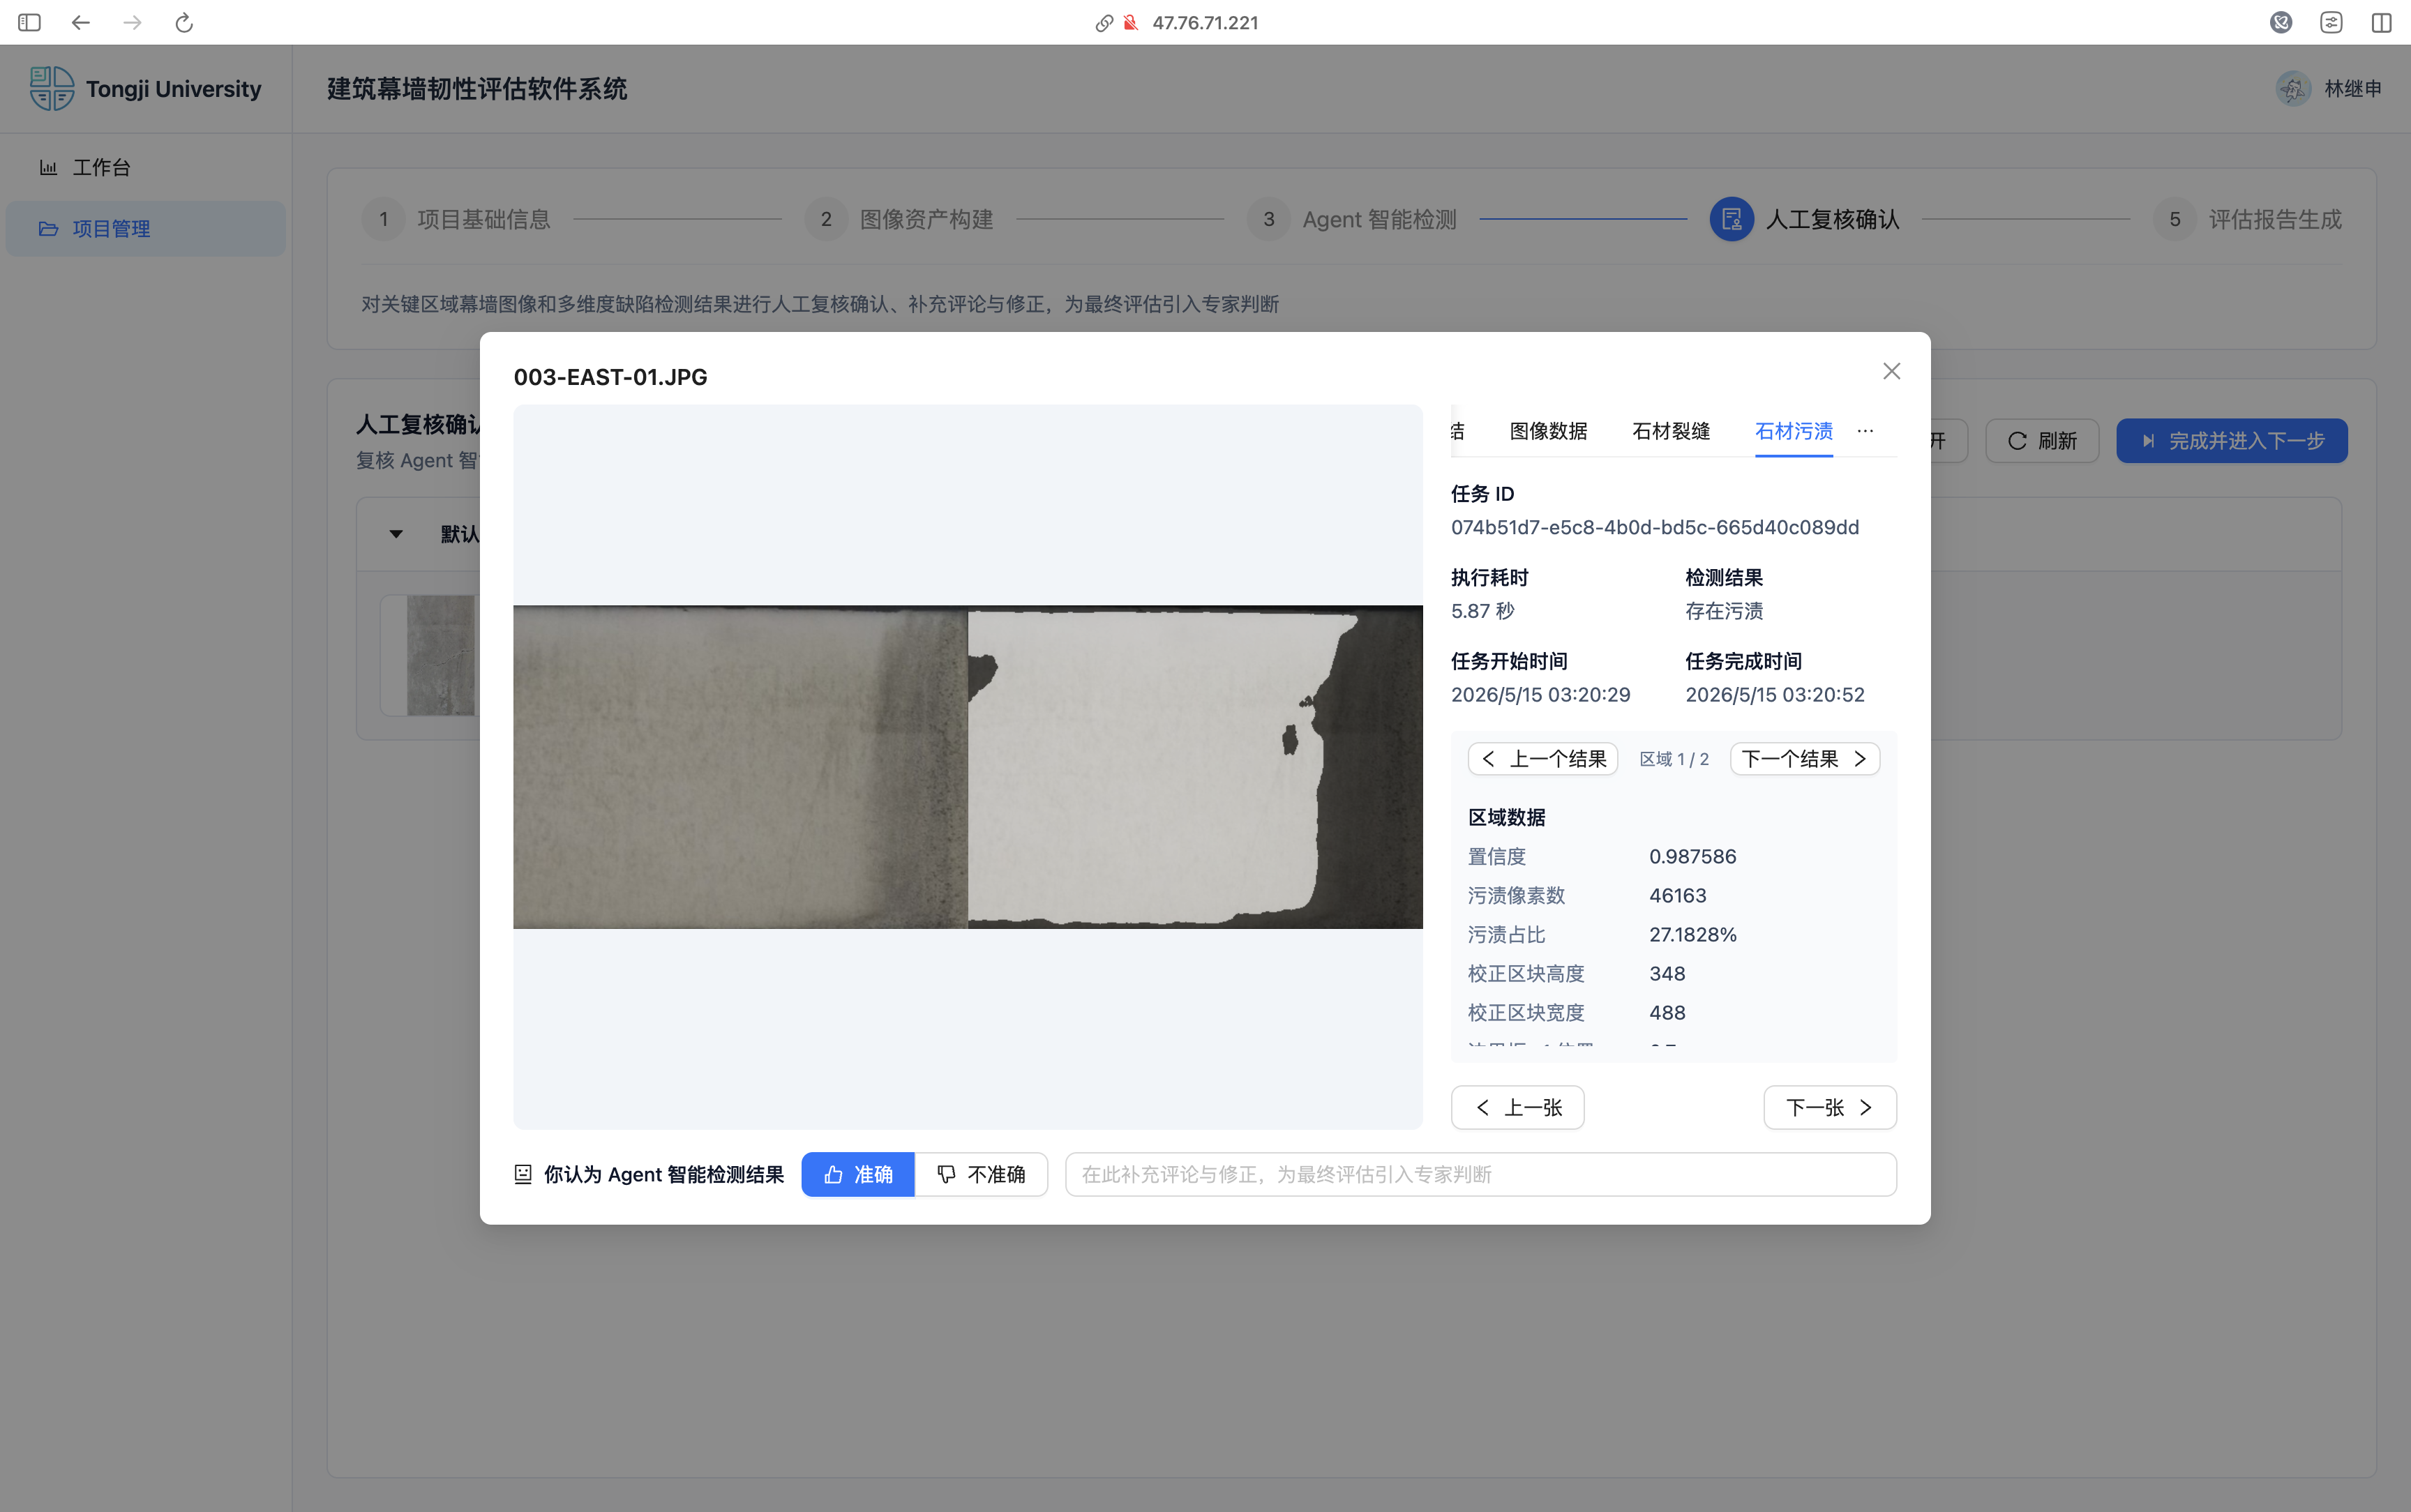
\includegraphics[width=0.95\textwidth]{figures/showcase_09_stain_detection.png}
  \caption{石材污渍检测结果界面}
  \label{fig:validation-showcase-stain-detection}
\end{figure}

\begin{figure}[!htbp]
  \centering
  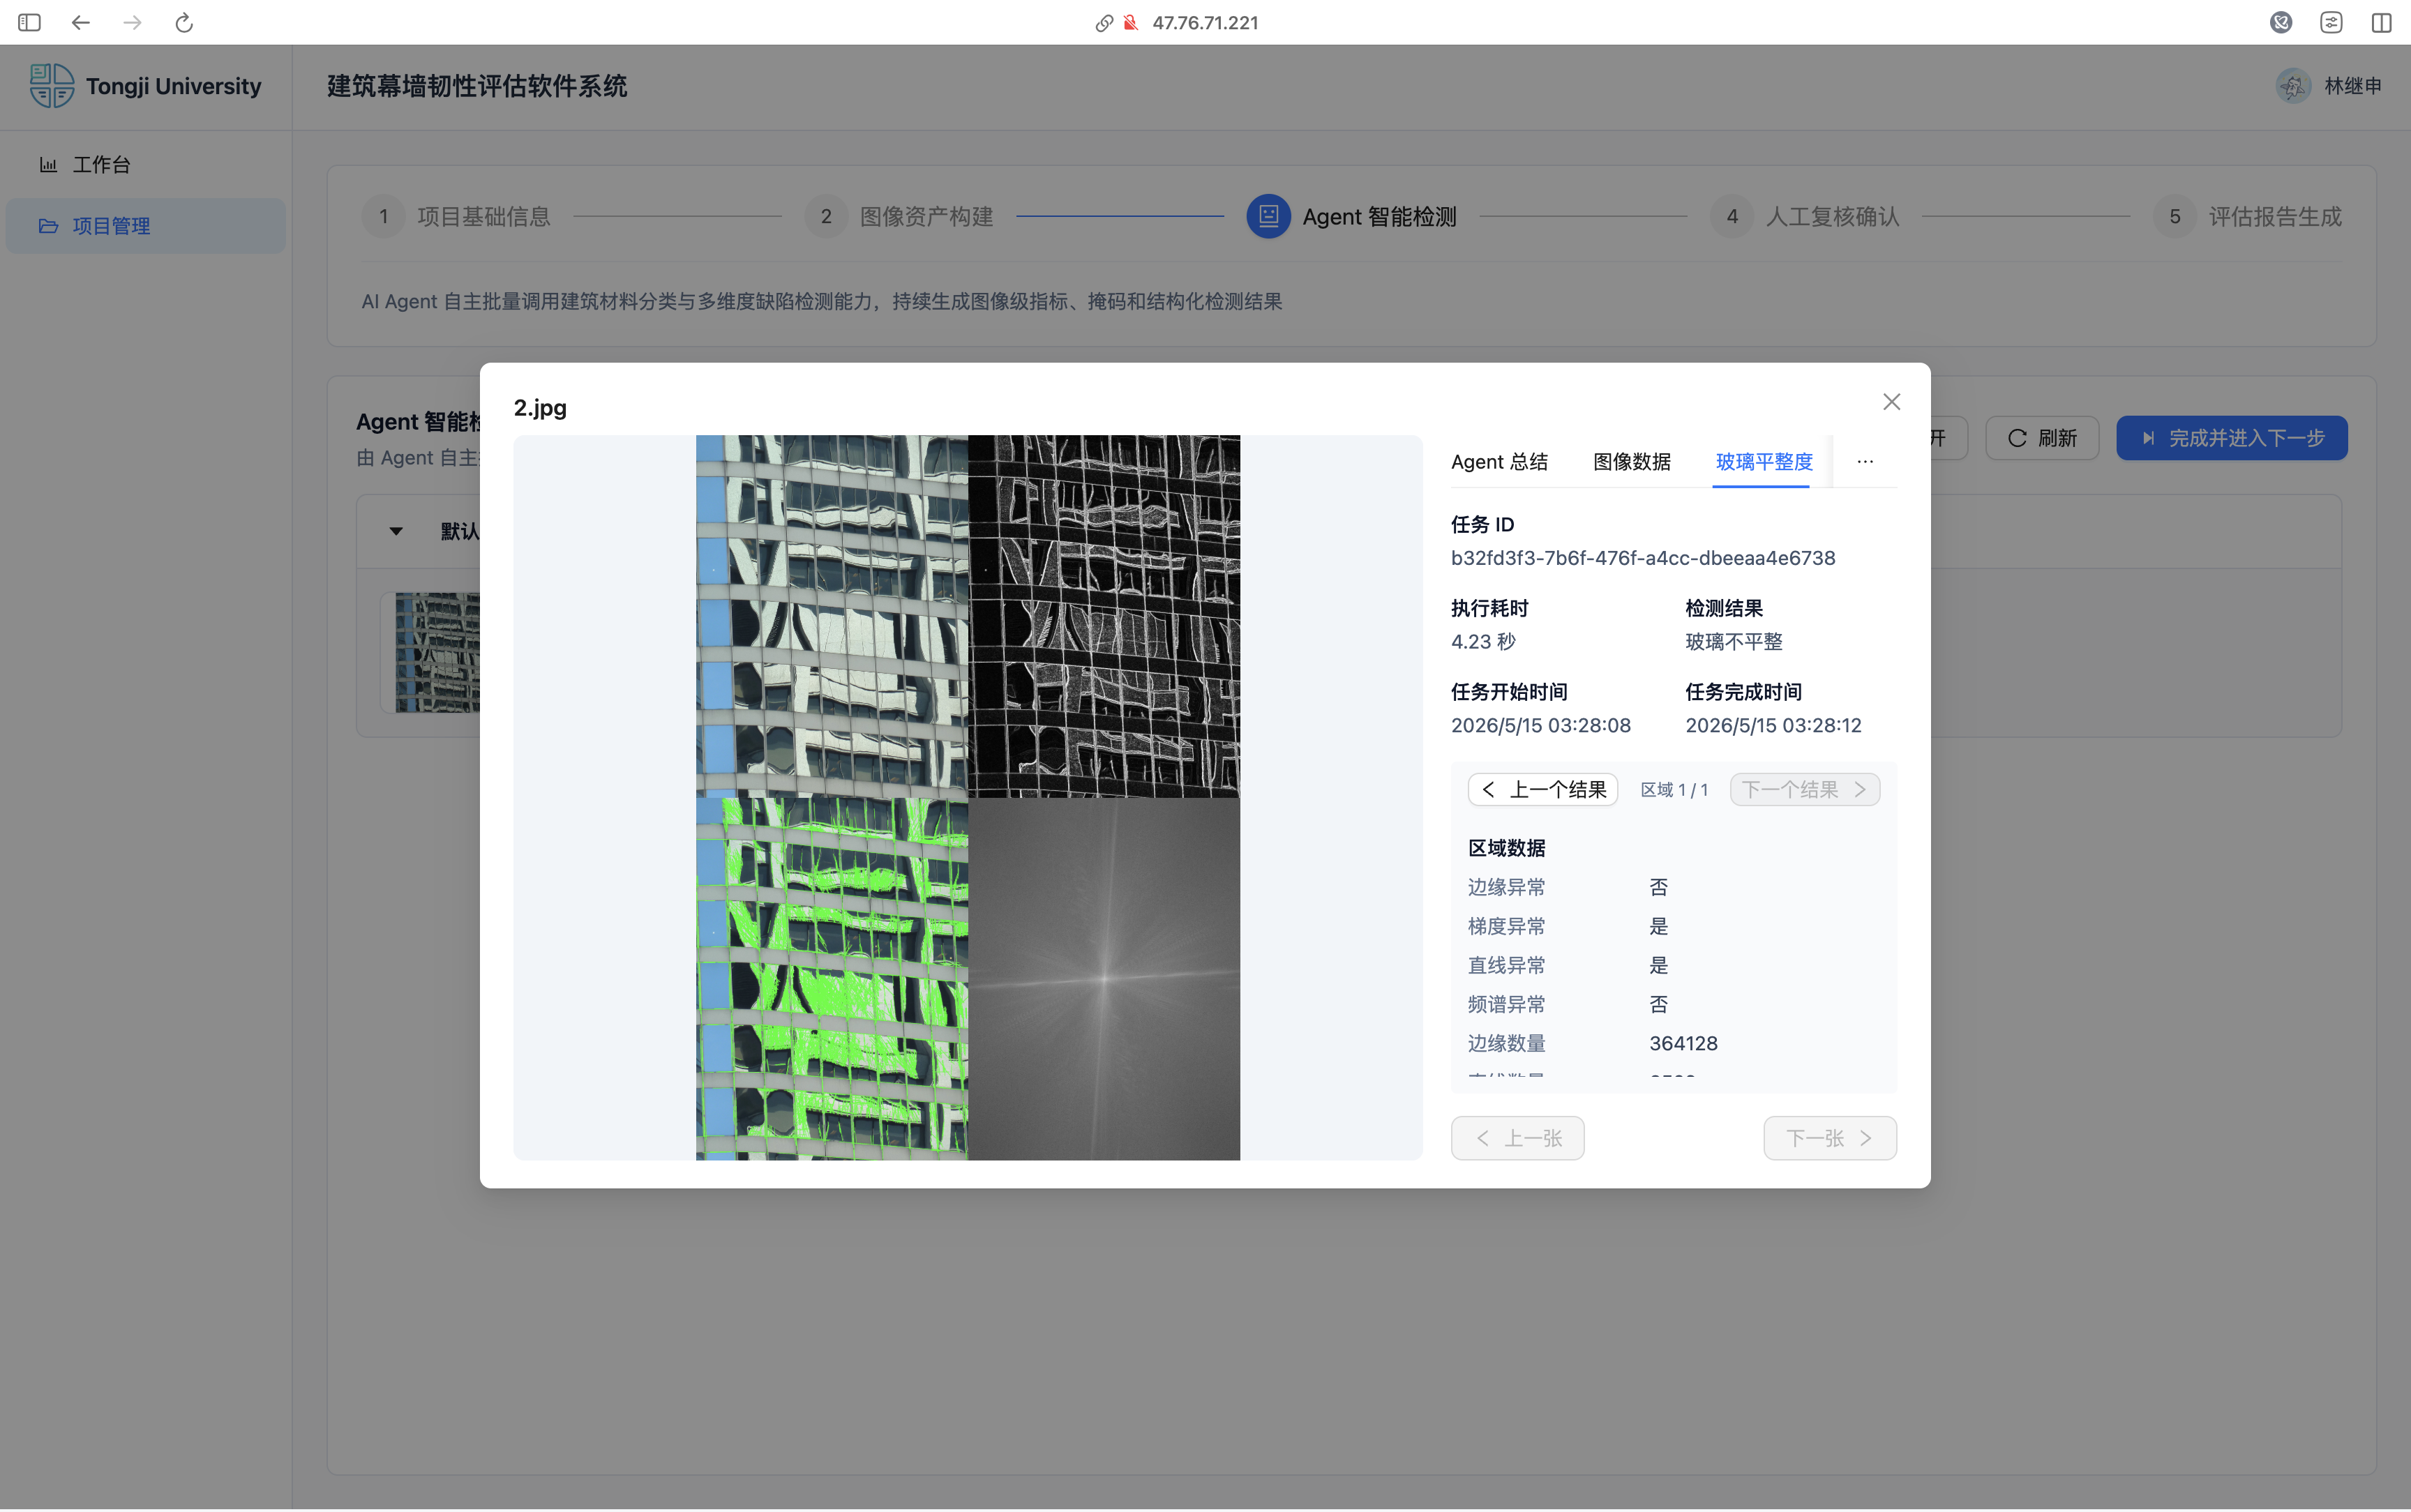
\includegraphics[width=0.95\textwidth]{figures/showcase_10_flatness_detection.png}
  \caption{玻璃平整度检测结果界面}
  \label{fig:validation-showcase-flatness-detection}
\end{figure}

\begin{figure}[!htbp]
  \centering
  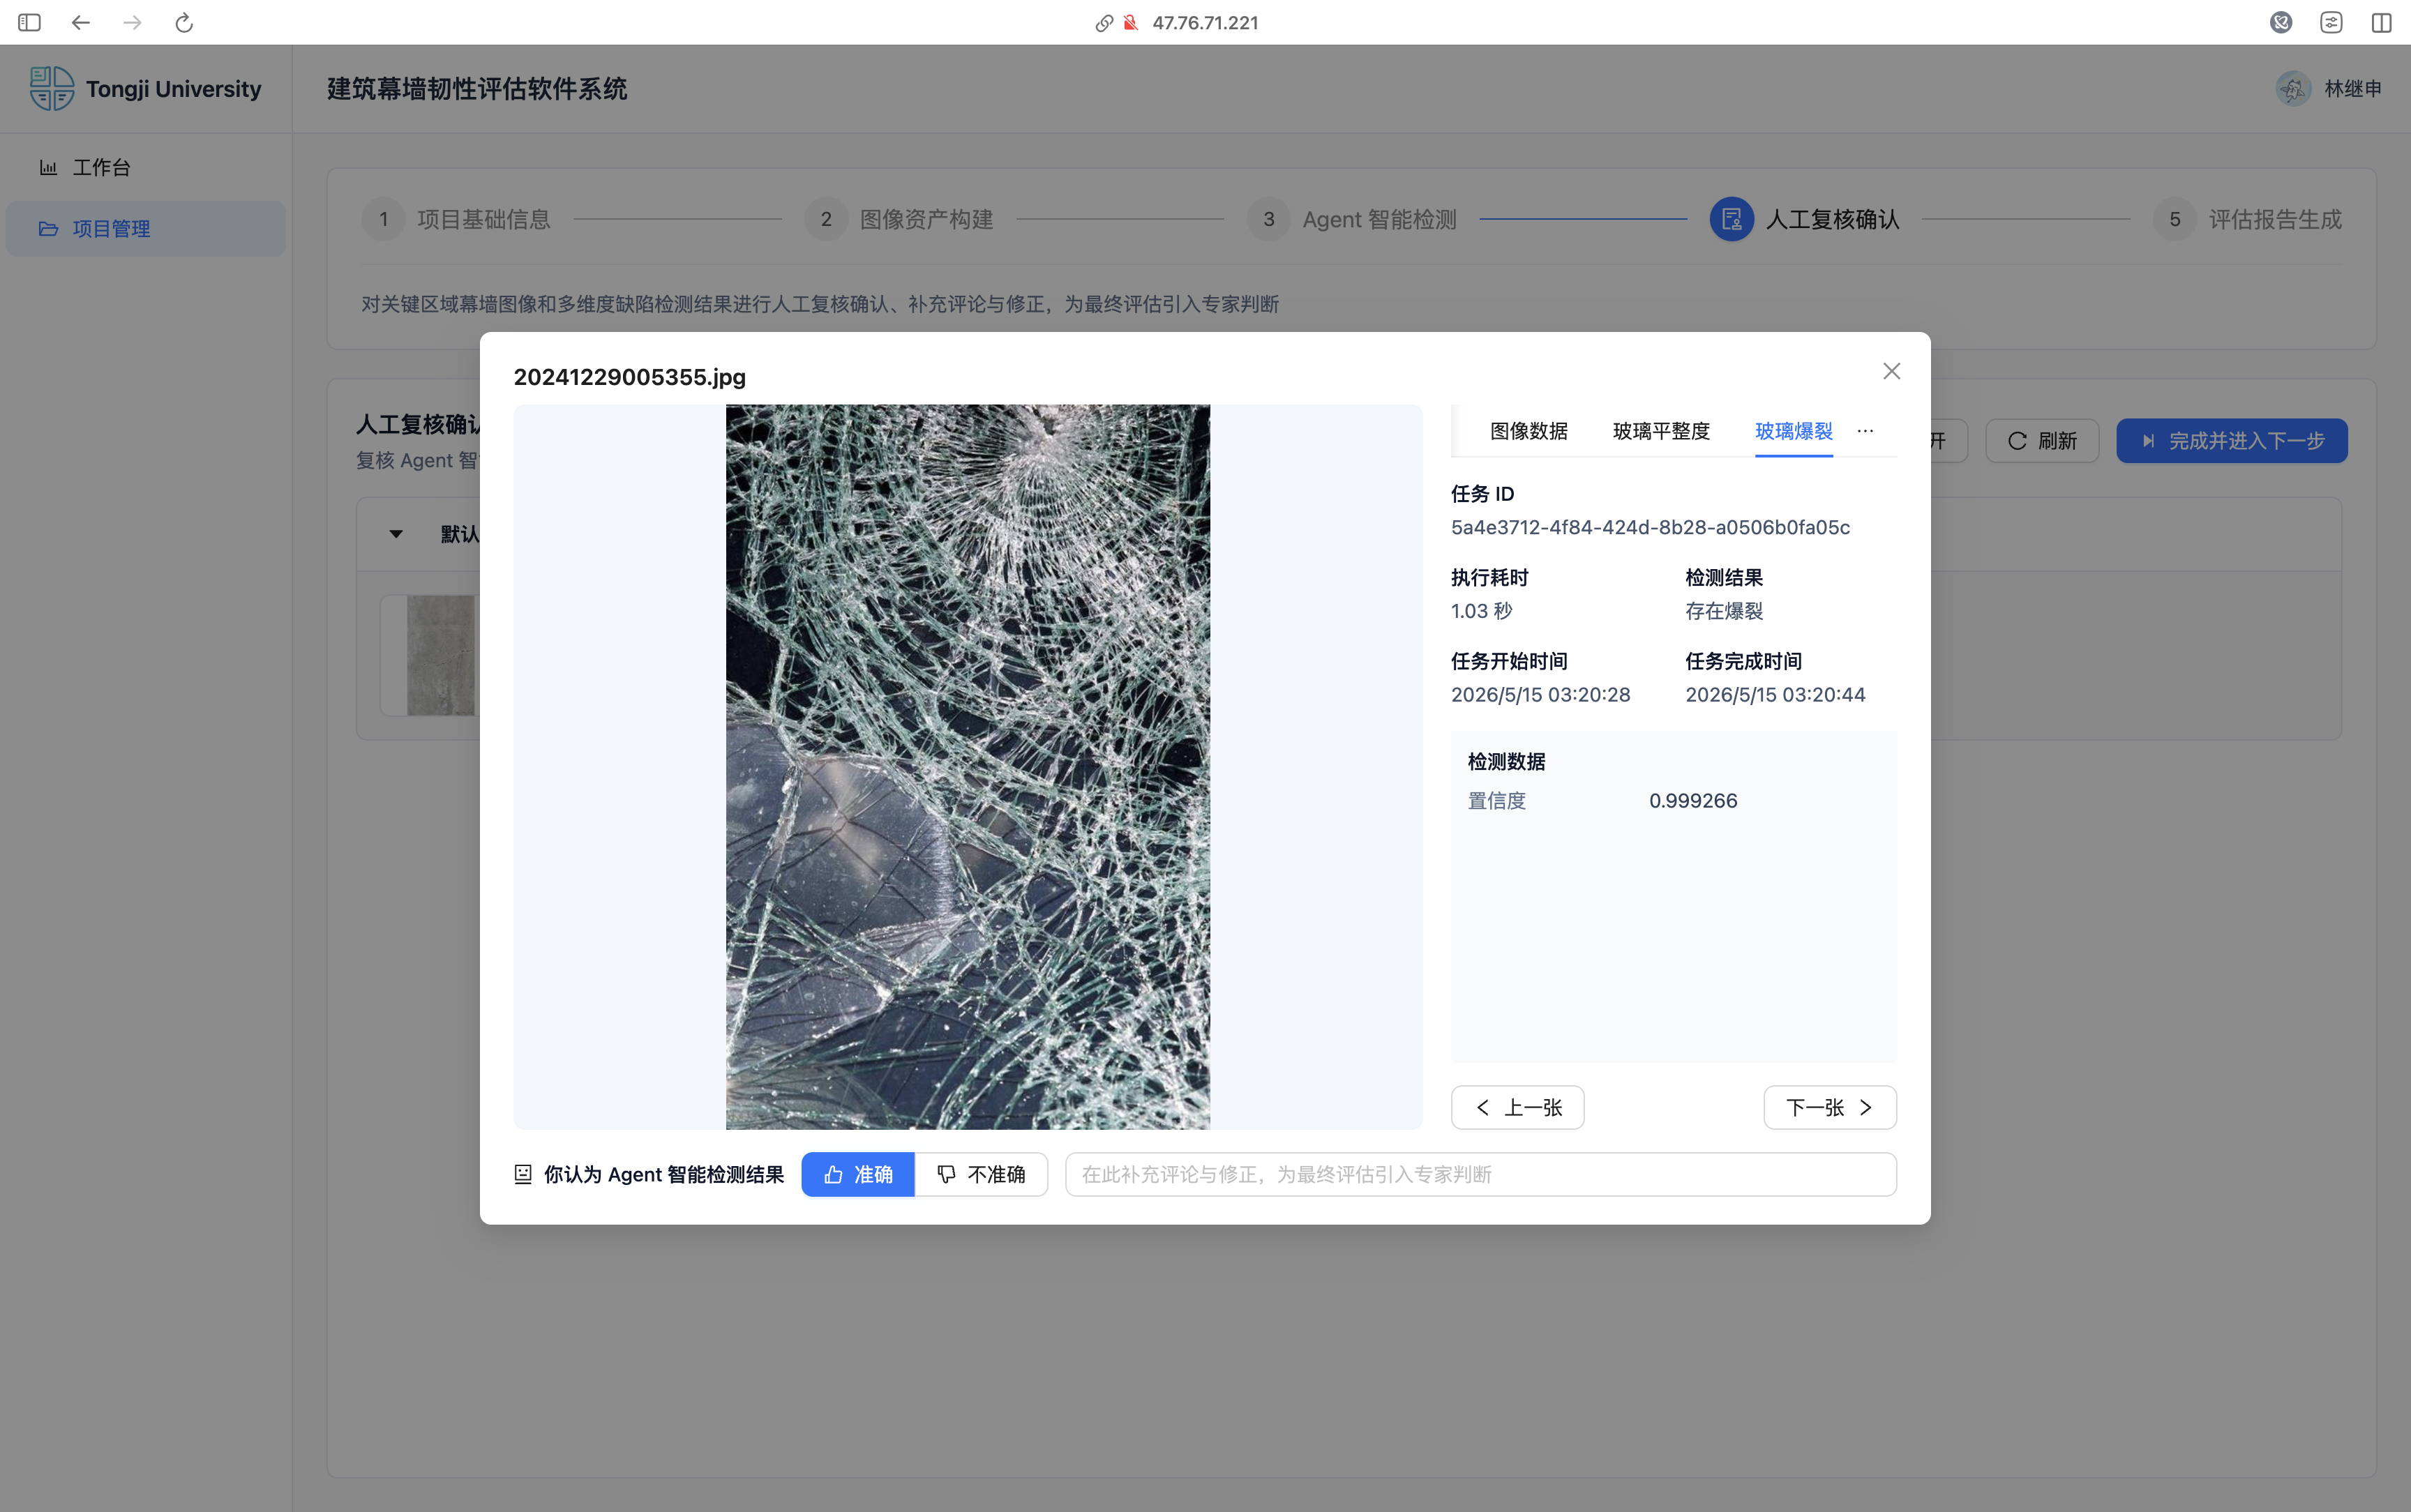
\includegraphics[width=0.95\textwidth]{figures/showcase_11_spalling_detection.png}
  \caption{玻璃爆裂检测结果界面}
  \label{fig:validation-showcase-spalling-detection}
\end{figure}

\subsection{LLM 分层信息整合策略验证结果}
\label{subsec:validation-llm-hierarchical-integration-result-display}

\begin{figure}[!htbp]
  \centering
  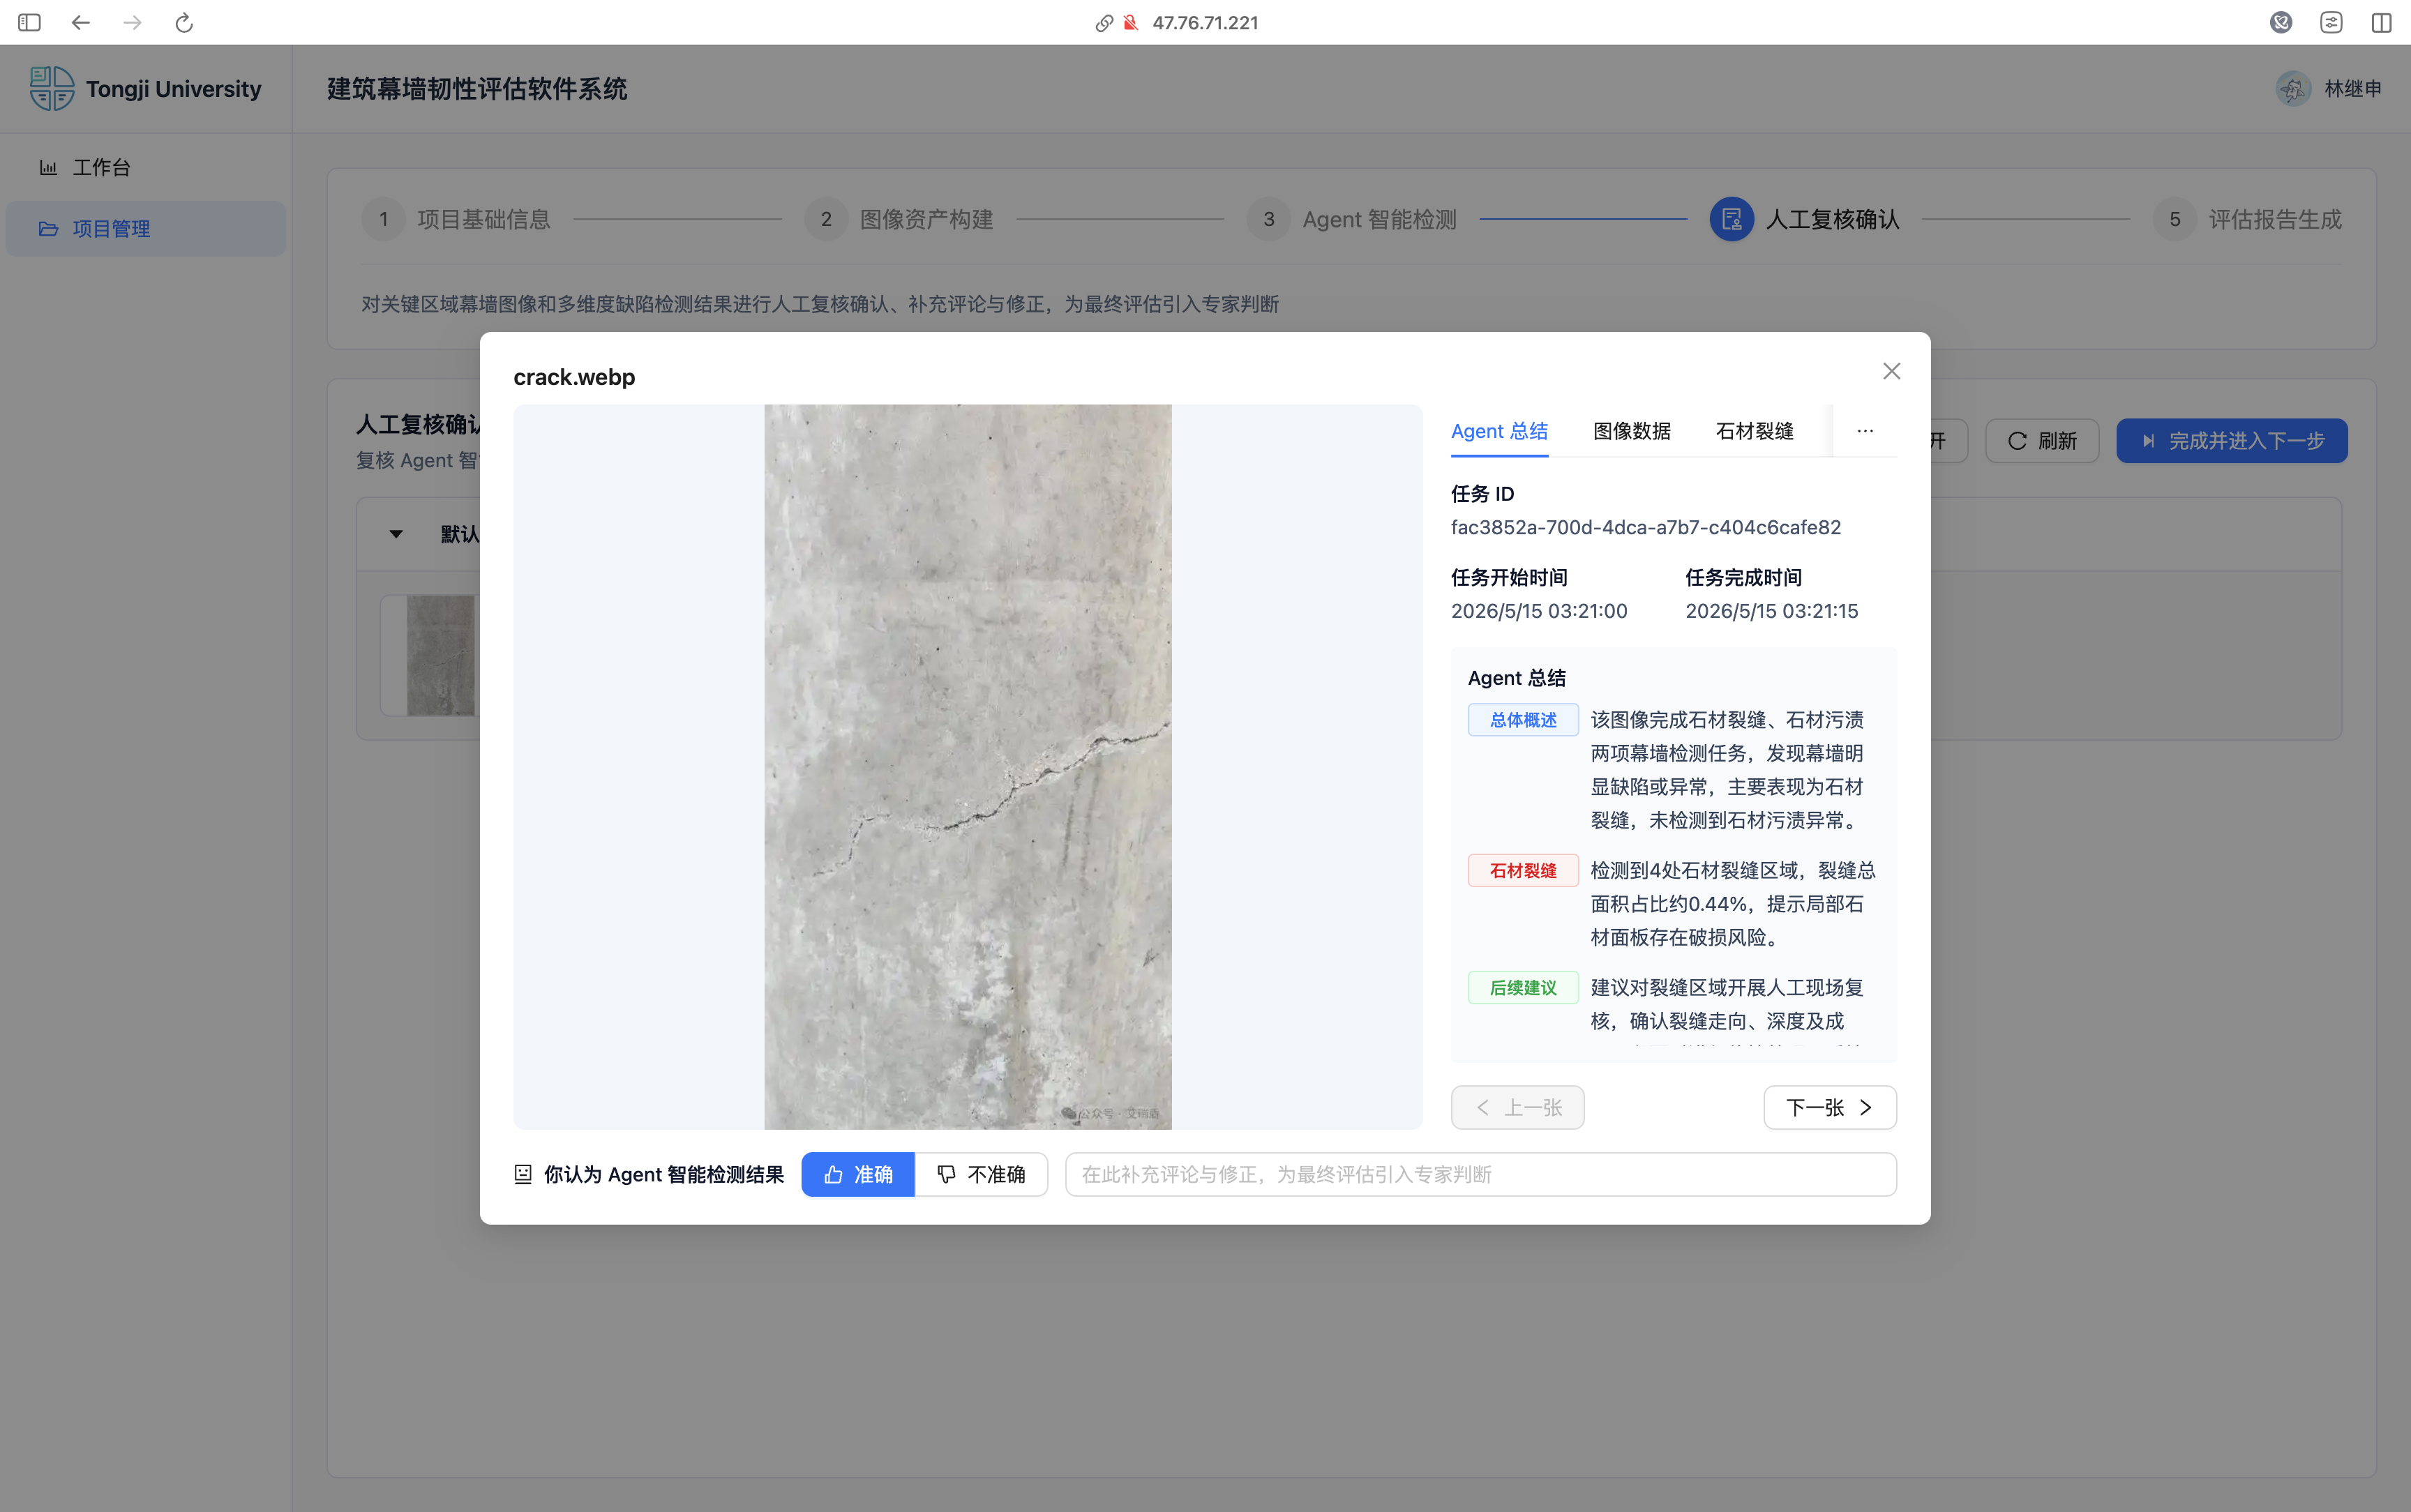
\includegraphics[width=0.95\textwidth]{figures/showcase_12_detection_summary.png}
  \caption{图像级 Agent 总结与人工复核界面}
  \label{fig:validation-showcase-detection-summary}
\end{figure}

\begin{figure}[!htbp]
  \centering
  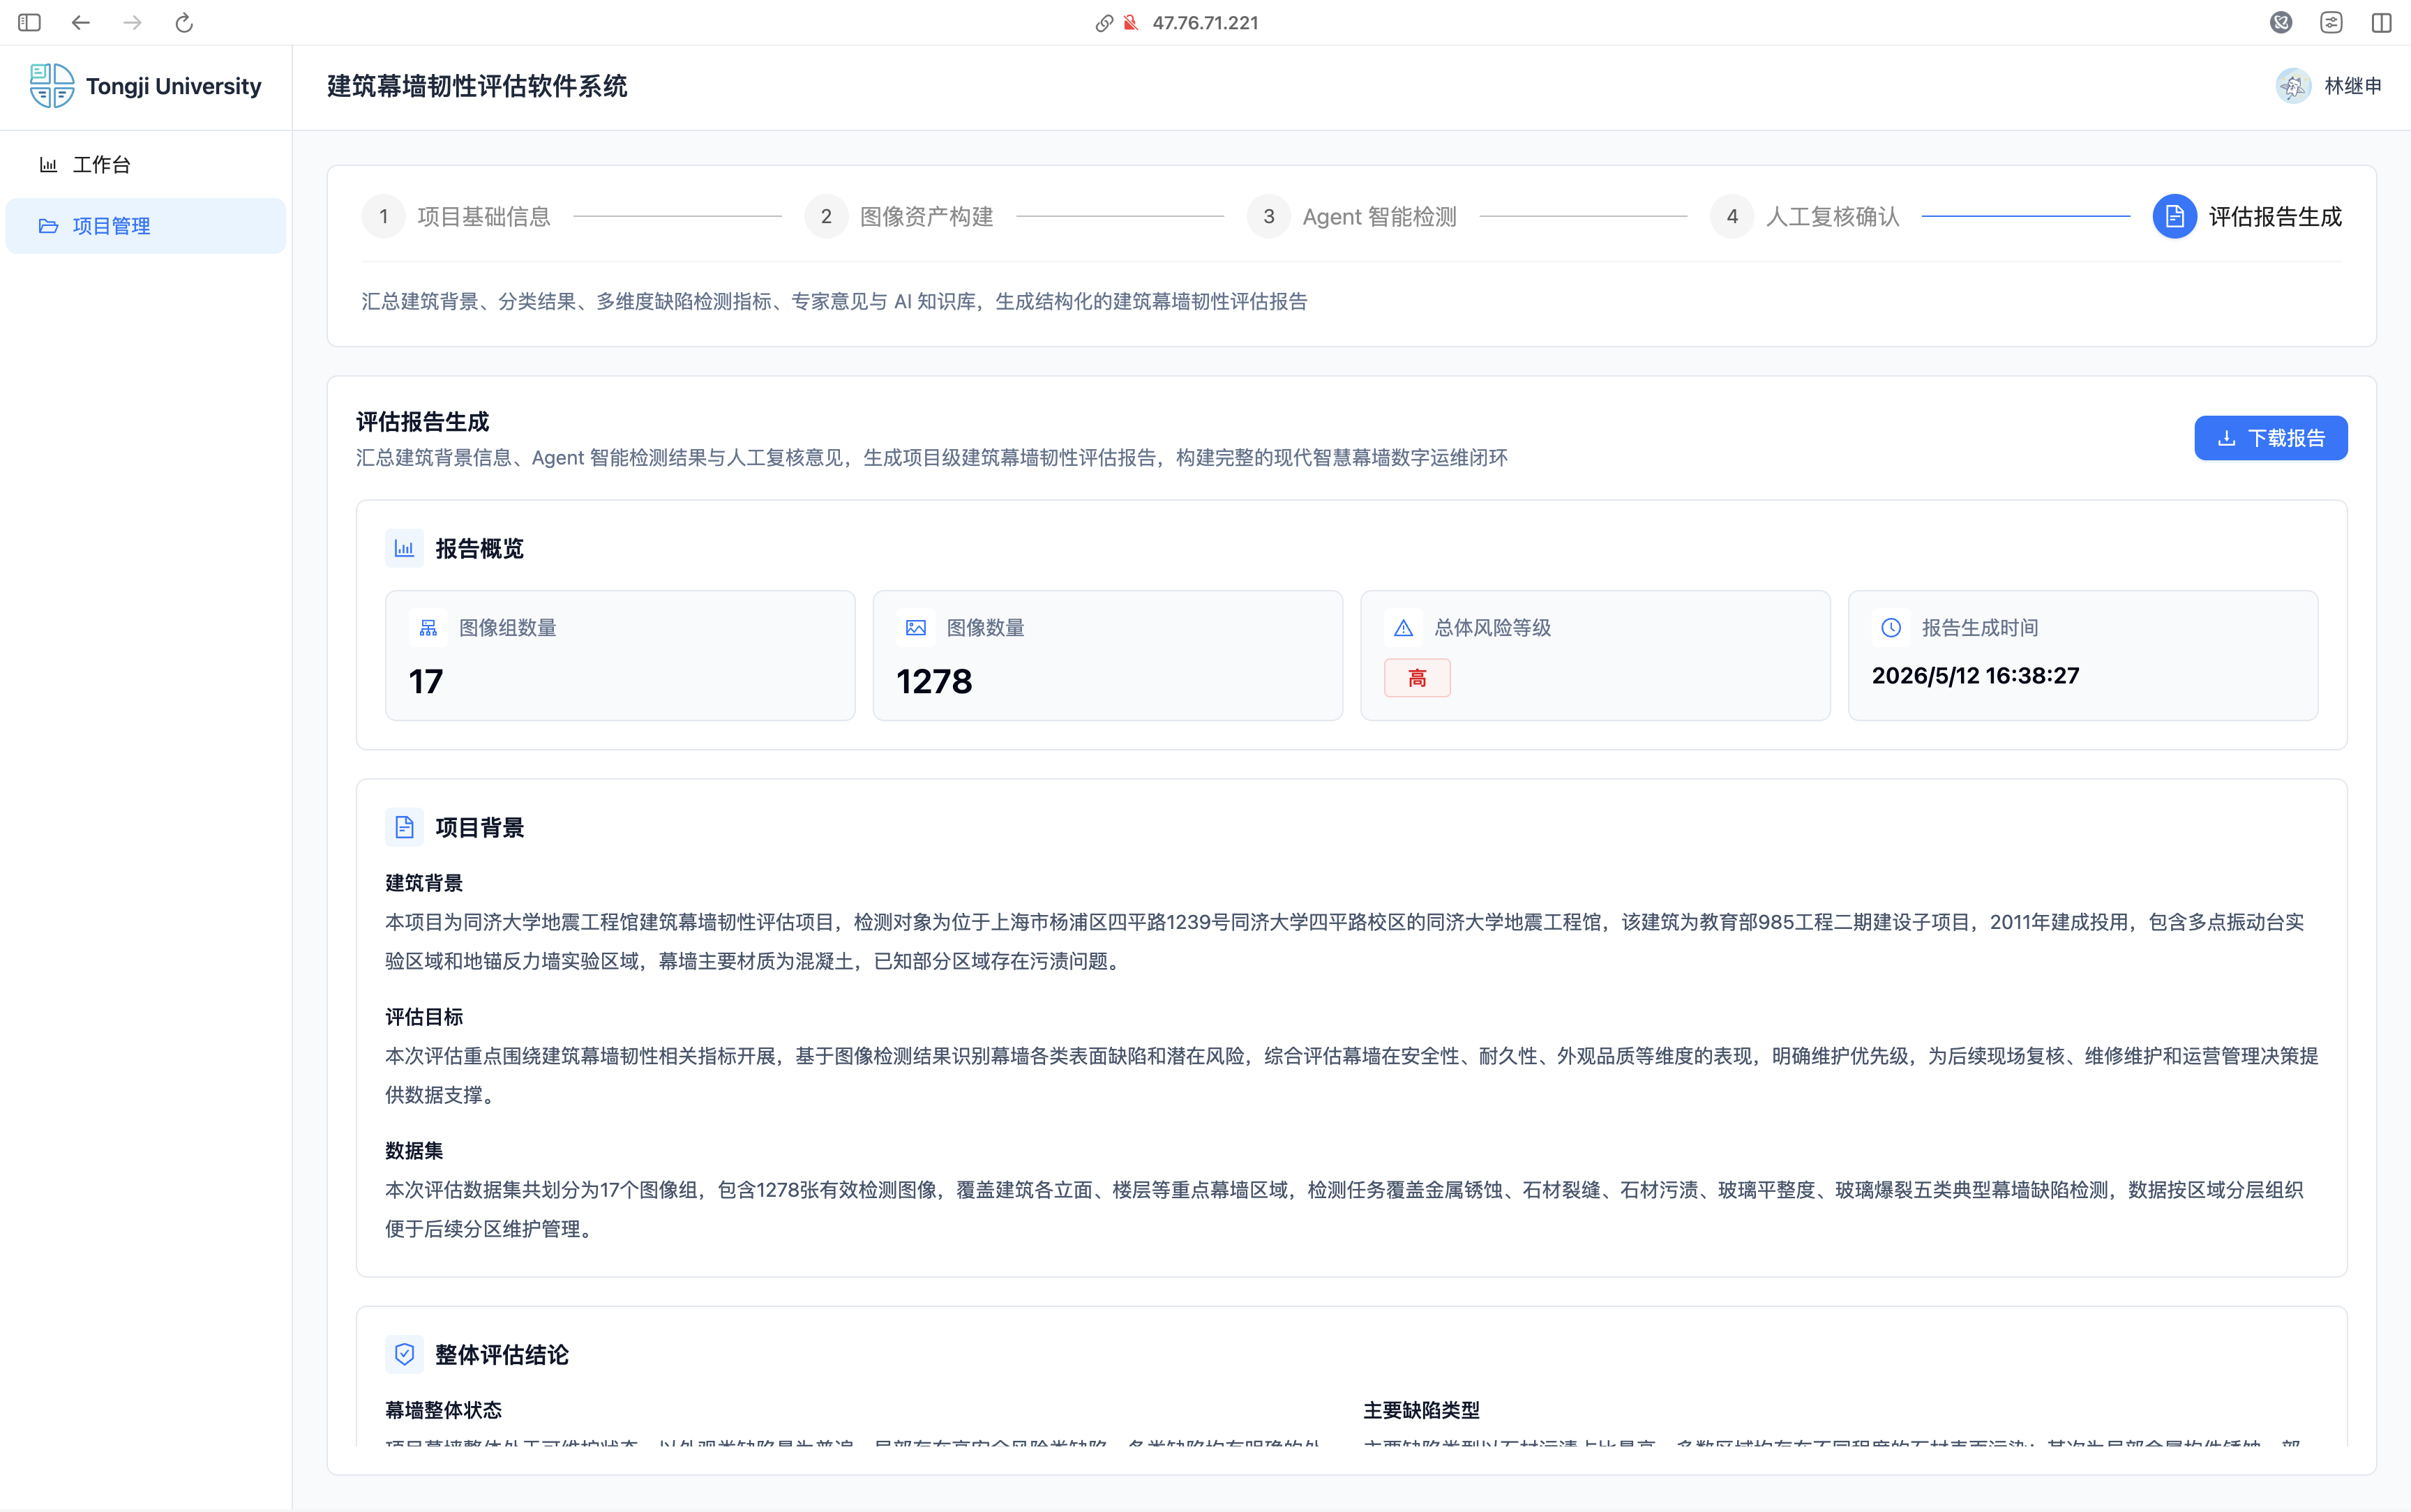
\includegraphics[width=0.95\textwidth]{figures/showcase_13_project_summary.png}
  \caption{项目韧性评估报告界面（一）}
  \label{fig:validation-showcase-project-summary-1}
\end{figure}

\begin{figure}[!htbp]
  \centering
  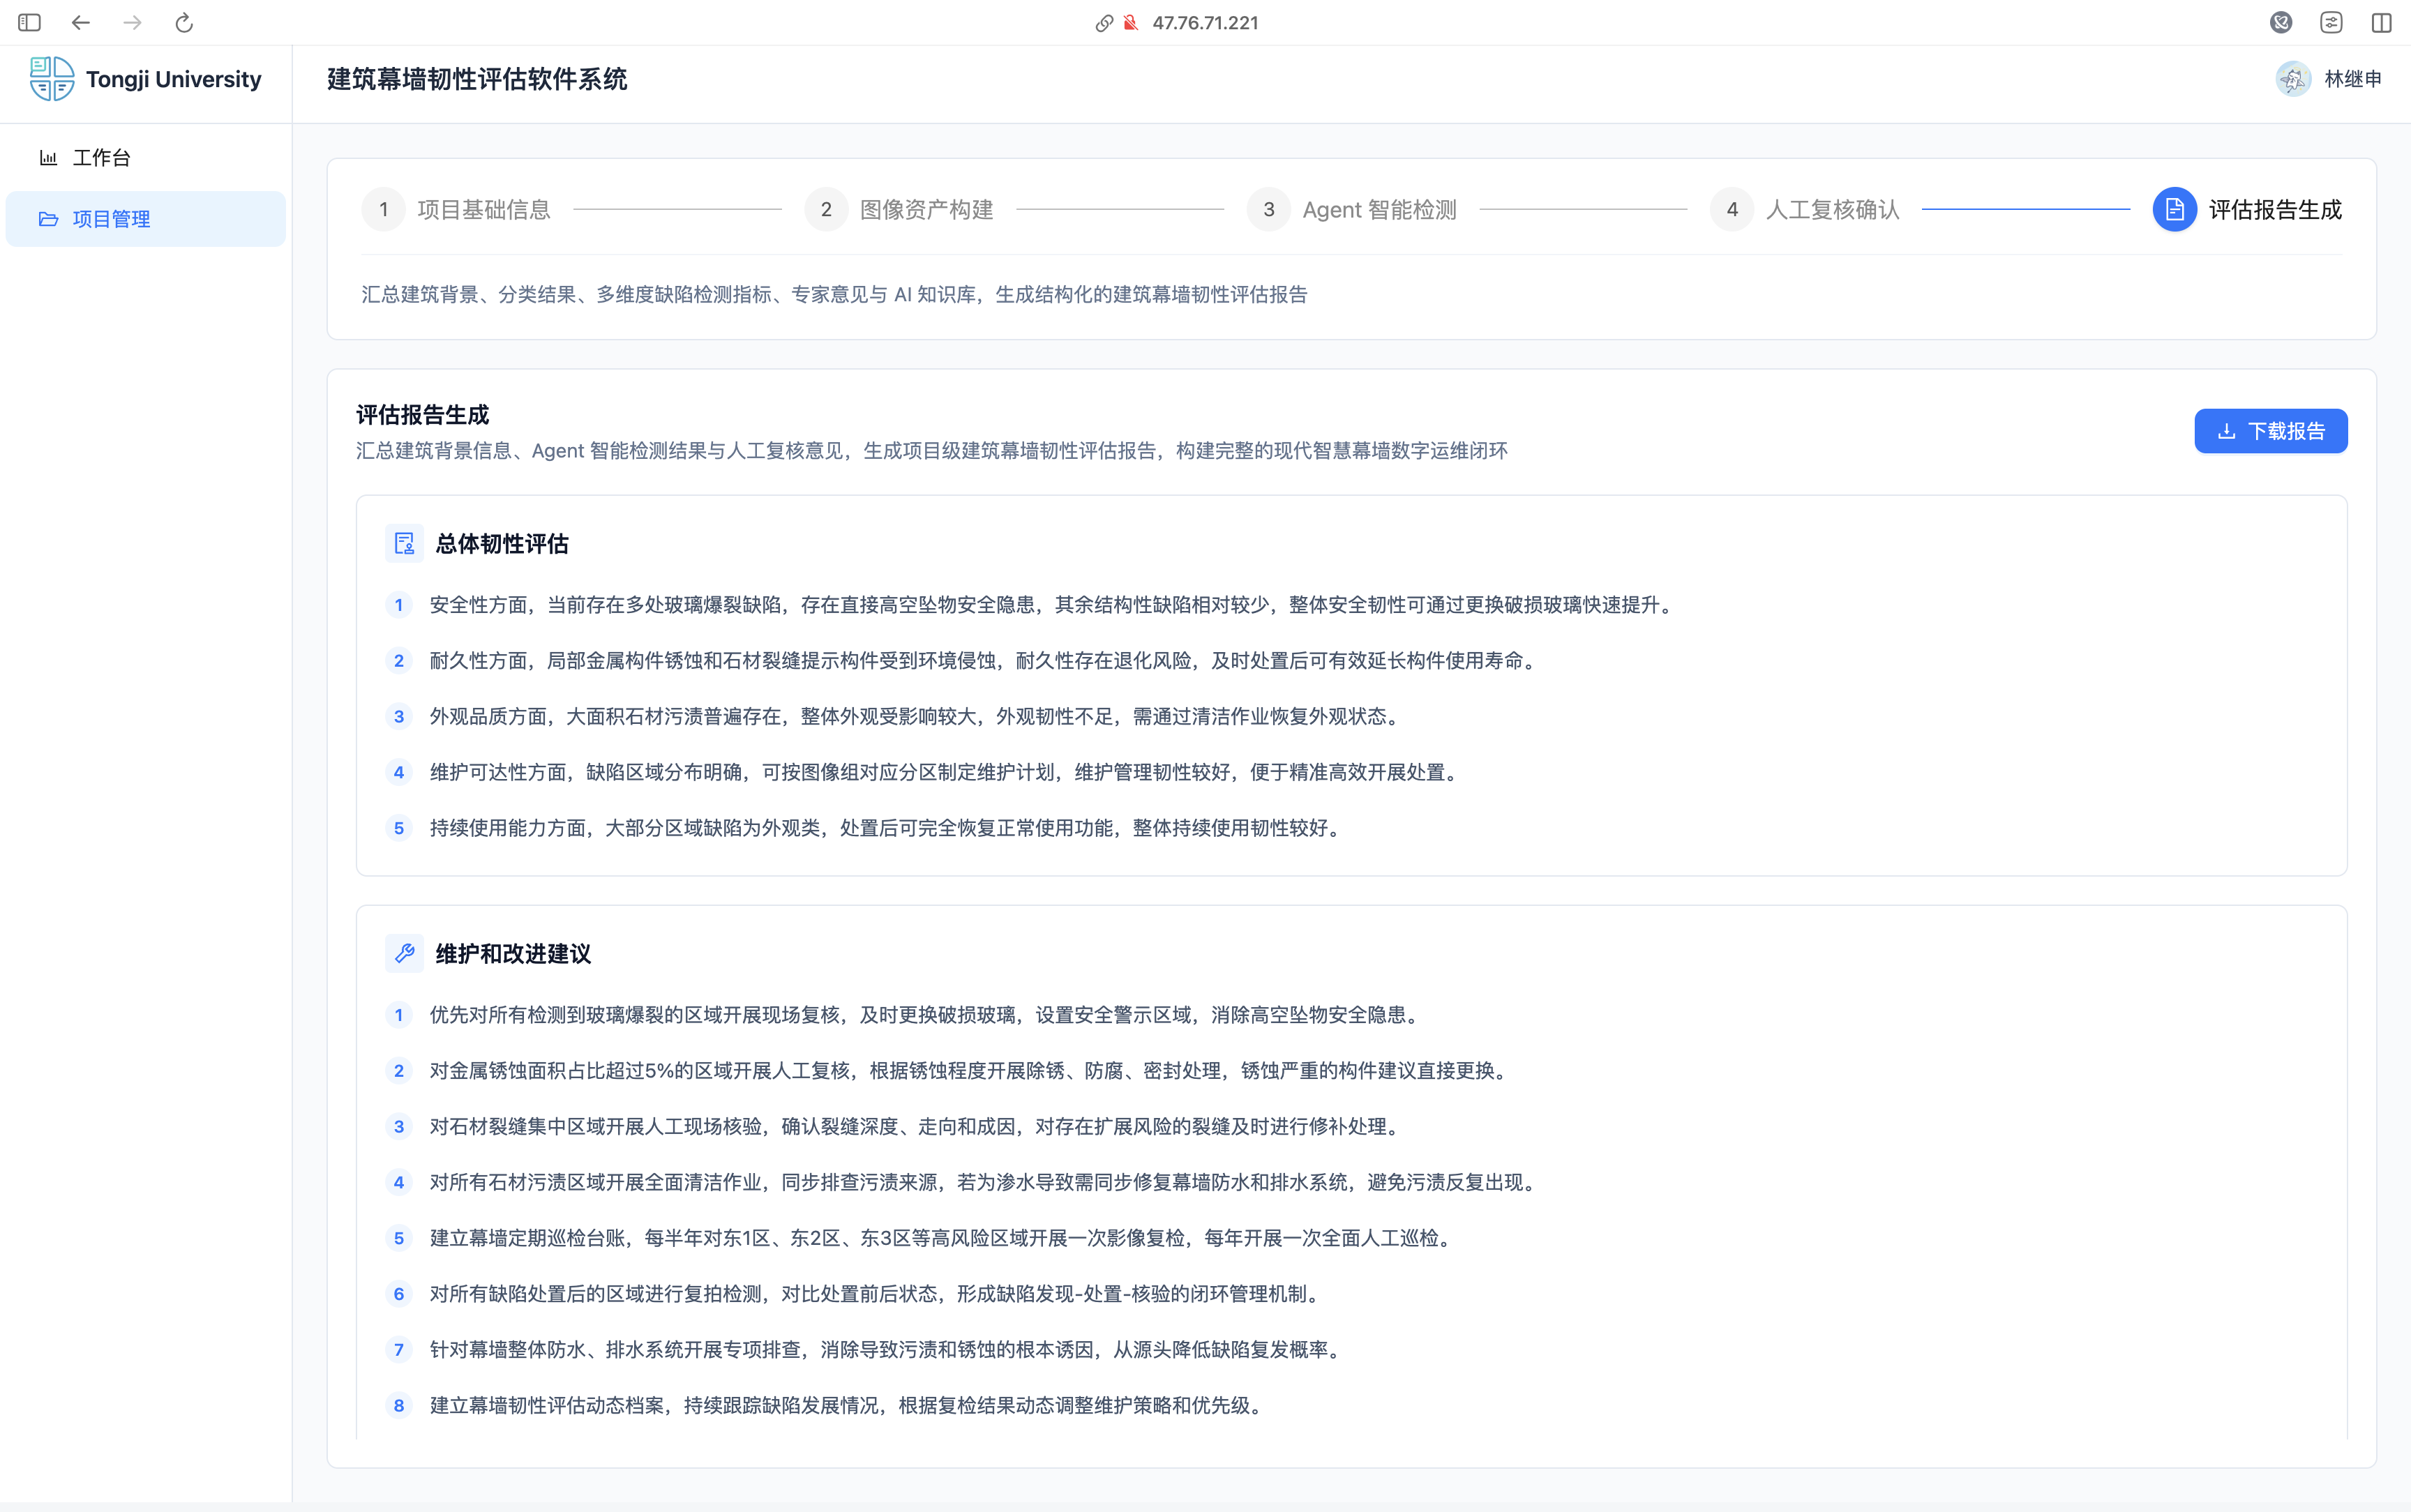
\includegraphics[width=0.95\textwidth]{figures/showcase_14_project_summary.png}
  \caption{项目韧性评估报告界面（二）}
  \label{fig:validation-showcase-project-summary-2}
\end{figure}

\subsection{状态一致性验证结果}
\label{subsec:validation-state-consistency-result-display}

状态一致性验证结果主要体现在检测进度、检测子任务状态、图像级总结状态、人工复核结果和报告生成状态的连续展示中。上述界面中，\cref{fig:validation-showcase-project-detection} 展示了 Agent 智能检测阶段的任务进度和节点状态，\cref{fig:validation-showcase-detection-summary} 展示了图像级总结与人工复核状态，\cref{fig:validation-showcase-project-summary-1,fig:validation-showcase-project-summary-2} 展示了项目报告生成后的前端结果。页面刷新和 WebSocket 增量更新均以数据库状态为准，因此这些界面共同体现了系统的状态一致性。

\subsection{部署验证结果}
\label{subsec:validation-deployment-result-display}

部署验证结果主要体现为 Docker Compose 环境下各服务能够完成启动、依赖初始化、服务名互访、对象存储访问、消息事件消费和前端页面访问。前述登录、工作台、项目管理、检测和报告界面均来自部署后的系统运行结果，说明 Core Web、Core API、Core BIZ、Activity 服务、RocketMQ、对象存储和日志采集等部署单元能够协同工作。

从这些界面可以看到，系统已经不只是一个模型调用入口，而是形成了项目级评估软件的基本形态。用户可以从工作台进入项目，维护项目资料，上传并组织图像，启动 Agent 智能检测，查看检测进度和检测结果，完成复核，最后生成项目级韧性评估报告。

\section{应用价值分析}
\label{sec:validation-application-value-analysis}

\begin{table}[!htb]
  \caption{不同实现方案对比}\label{tab:solution-comparison}
  \centering
  \begin{tabular}{@{}p{0.16\linewidth}p{0.25\linewidth}p{0.25\linewidth}p{0.25\linewidth}@{}} \toprule
    \textbf{方案} & \textbf{主要特点} & \textbf{适用范围} & \textbf{本文系统体现} \\ \midrule
    人工巡检 & 专家经验强，判断灵活 & 现场核验、经验判断和最终处置决策 & 用系统管理图像与流程，辅助形成结构化评估依据 \\
    单模型检测 & 对单类缺陷识别直接有效 & 单张图像、单类缺陷和局部结果判断 & 将模型封装为 Agent 可调度的原子检测能力 \\
    端到端大模型报告 & 自然语言生成能力强 & 文本整理、语义归纳和报告表达 & 采用 LLM 分层信息整合策略和结构化落库 \\
    本文方案 & 可调度、可追踪、可复核、可报告 & 项目级图像资产管理和建筑级韧性评估 & 通过工程链路形成从图像资产到评估报告的软件闭环 \\ \bottomrule
  \end{tabular}
\end{table}

如\cref{tab:solution-comparison} 所示，本文系统将人工巡检经验、原子检测能力和大模型文本生成能力组织到同一条工程链路中。相比只关注单张图像的检测工具，系统进一步形成了项目、图像、检测、总结、复核和报告之间的连续关系；相比只生成文本的报告工具，系统保留了结构化证据、任务状态和产物追踪。结合实际部署与试用情况，系统已经能够支持建筑幕墙巡检图像的统一管理、智能检测、人工复核和报告生成，为建筑幕墙数字运维提供了可实施的软件原型。

从应用角度看，本系统的价值主要体现在幕墙巡检、缺陷检测和报告生成三个环节。对于幕墙巡检中数量较多、来源较分散的图像，系统能够按项目和图像组进行管理，后续查找、复核和区域化分析都会更方便。Agent 自主任务调度方法则减少了人工判断检测能力的步骤，系统可以根据图像内容选择合适的检测任务，而不是让用户逐项手动指定。检测结束后，LLM 分层信息整合策略把底层指标、图像级总结和复核意见逐步整理为项目报告，能够减轻人工汇总报告的工作量。实时进度和结果可视化也让用户更容易理解长任务正在执行到哪一步，失败时也能知道需要从哪里重新处理。

单一检测工具通常只能回答某张图像是否存在某类缺陷，而本文系统更关注运维场景中的连续流程：项目如何建立，图像如何组织，检测任务如何执行，结果如何复核，报告又如何生成。与纯 Agent 应用相比，本系统没有让 Agent 直接决定数据库状态，而是通过任务代码、状态机和接口协议进行约束。这样既保留了 Agent 在语义判断和信息整理上的作用，也使系统更接近真实软件系统的运行方式。

\section{本章小结}
\label{sec:validation-chapter-summary}

本章围绕系统功能、Agent 自主任务调度方法、LLM 分层信息整合策略、状态一致性和部署过程对系统进行了验证。验证结果说明，系统能够从项目级图像资产出发，经过智能检测、人工复核和报告生成，形成建筑幕墙韧性评估报告。分类 Agent 的输出会真实改变后续检测任务，图像级总结和项目级报告也能够在结构化数据基础上逐步生成。与此同时，状态机、消息队列、WebSocket 和 Docker Compose 部署共同支撑稳定的工程链路。通过本章验证，可以说明该软件原型系统能够支撑从项目级图像资产到建筑韧性评估报告的完整业务流程。
